\chapter{Experimentos}
\label{cap:capitulo6}

\vspace{1cm}

En este capítulo se presentan las diferentes pruebas realizadas para validar el funcionamiento de los distintos módulos del proyecto. Los experimentos realizados permiten evaluar el comportamiento del sistema de dispensación, la comunicación entre el dispositivo y la aplicación móvil, el funcionamiento del pulsómetro y los mecanismos de almacenamiento y seguridad implementados, verificando que el sistema cumple los requisitos establecidos durante las fases de diseño y desarrollo.


\section{Sistema de dispensación}

El sistema de dispensación constituye uno de los elementos fundamentales del dispositivo, ya que es el encargado de posicionar los compartimentos del carrusel y garantizar la correcta liberación de las dosis programadas. Debido a su importancia dentro del funcionamiento global del sistema, se realizaron diferentes pruebas orientadas a validar el comportamiento del mecanismo y comprobar su fiabilidad durante el proceso de dispensación.

\subsection{Ajuste del mecanismo de dispensación}

Antes de validar el funcionamiento integral del sistema de dispensación, fue necesario calibrar y ajustar los elementos mecánicos responsables del movimiento del carrusel. El propósito de este paso fue asegurar que se alinease correctamente cada compartimento con la salida de dispensación en cada toma programada.\\

Durante las primeras pruebas del mecanismo se observó que pequeños aspectos como la holgura en el movimiento del carrusel o la altura a la que el trinquete tenía contacto con el impulsor del servo, afectaban al correcto comportamiento del mecanismo de dispensación.\\

Debido a ello, se realizaron sucesivos ajustes, como modificar la altura a la que se posicionaba el trinquete, y el diseño del impulsor del servo para mejorar la transmisión del movimiento. La Figura~\ref{fig:impulsores} muestra la evolución de los diferentes diseños desarrollados durante esta fase.

\begin{figure}[H]
    \centering
    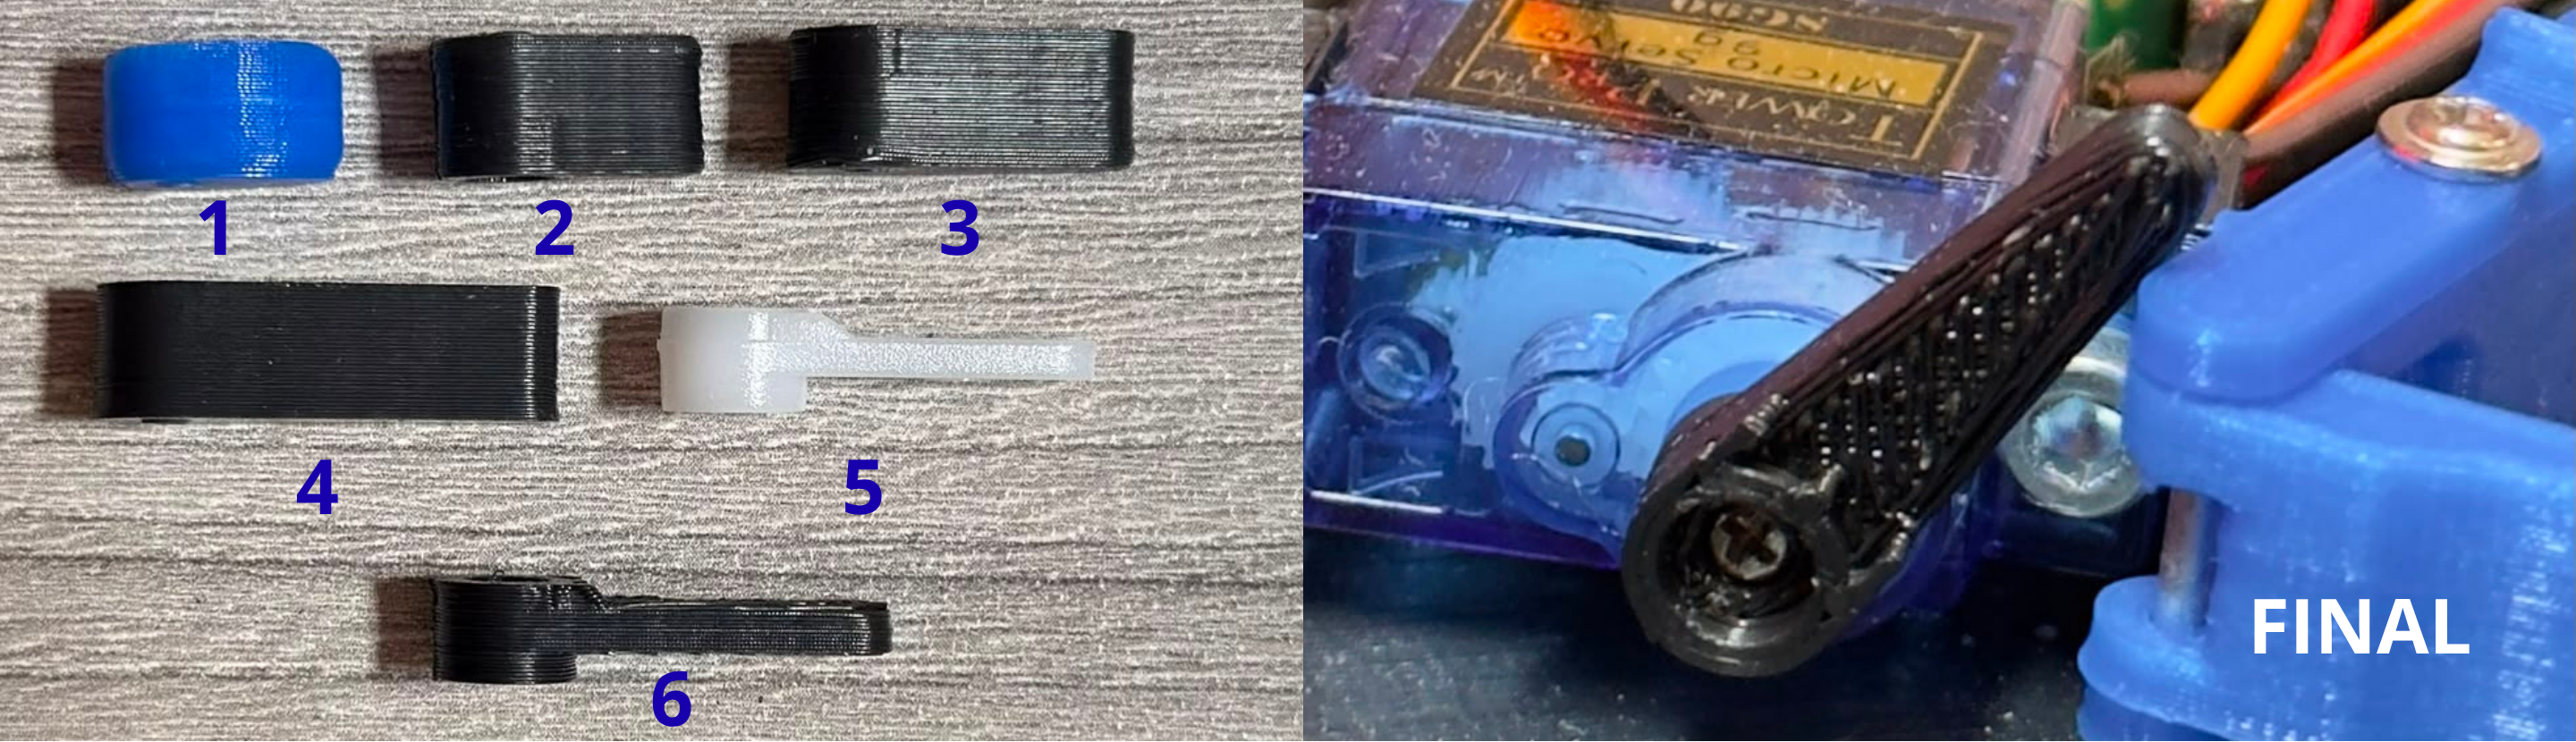
\includegraphics[width=\textwidth]{figs/collage_impulsores.png}
    \caption{Evolución del diseño del impulsor del servomotor}
    \label{fig:impulsores}
\end{figure}

Además, se incorporó un elemento de apoyo para reducir la libertad de movimiento del carrusel durante la rotación y se reajustó la posición del muelle de retorno para asegurar que el trinquete recuperase su posición de inicio adecuadamente tras cada accionamiento. Las principales modificaciones se pueden ver en la Figura~\ref{fig:modificaciones}.

\begin{figure}[H]
    \centering
    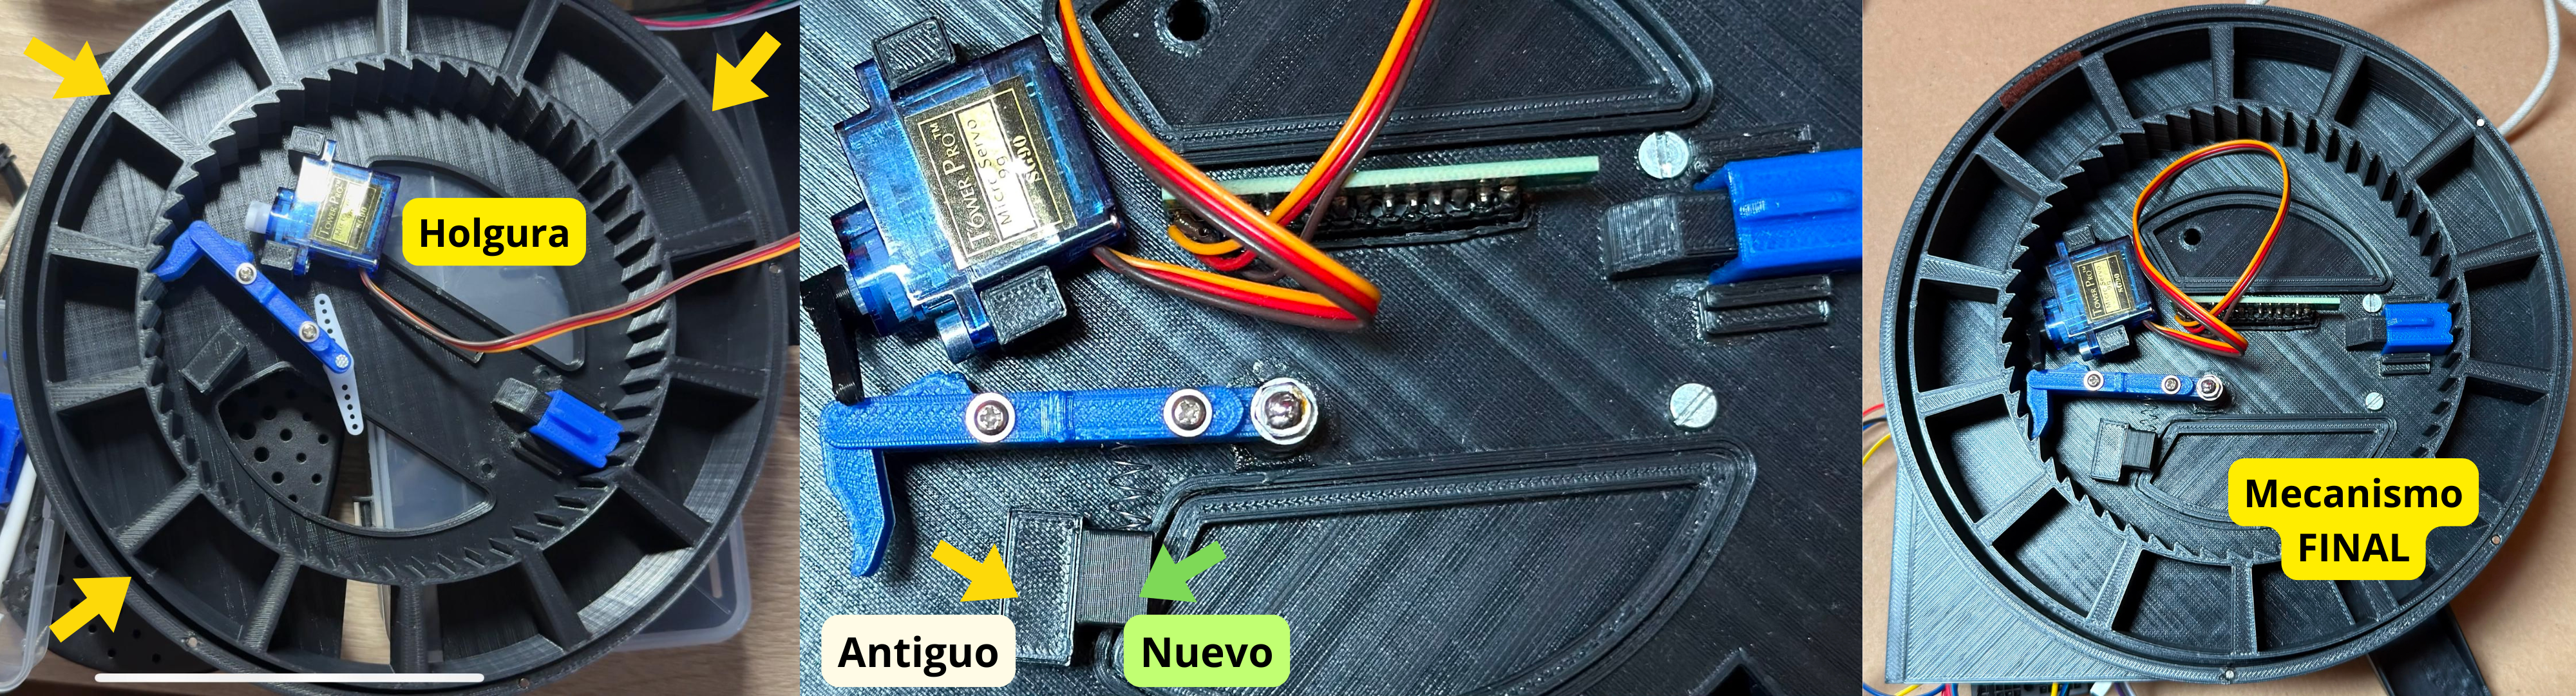
\includegraphics[width=\textwidth]{figs/modificaciones.png}
    \caption{Principales modificaciones realizadas durante el ajuste del mecanismo de dispensación: holgura observada, modificación de la posición del muelle del trinquete y configuración final del mecanismo.}
    \label{fig:modificaciones}
\end{figure}

La metodología consistió en probar distintas combinaciones secuenciales de los cambios mencionados hasta verificar visualmente la alineación de los compartimentos con la salida de medicación y sin interferencias mecánicas en el movimiento.\\

Una vez completado el ajuste se establecieron las modificaciones posteriormente durante las pruebas de dispensación automática. Este método permitió que el sistema funcionara con una configuración mecánica estable antes de poner a prueba su desempeño en condiciones reales de uso.

\subsection{Validación del proceso de dispensación}

El objetivo de este experimento fue validar el funcionamiento completo del proceso de dispensación automática, verificando que las tomas programadas se ejecutan correctamente a la hora establecida.\\

La metodología seguida consistió, en primer lugar, en programar una toma desde la aplicación móvil y comprobar que era sincronizada correctamente con el dispensador. Posteriormente, se esperó a la hora programada para verificar la activación del servomotor correspondiente y la correcta dispensación del medicamento. Una vez completada la primera dispensación, se programó una segunda toma directamente desde la interfaz del dispositivo.\\

El desarrollo completo de la prueba puede observarse en el vídeo asociado\footnote{\url{https://tinyurl.com/3c78pjkb}}.
Los resultados obtenidos confirman el correcto funcionamiento del proceso de dispensación implementado.

\begin{figure}[H]
    \centering
    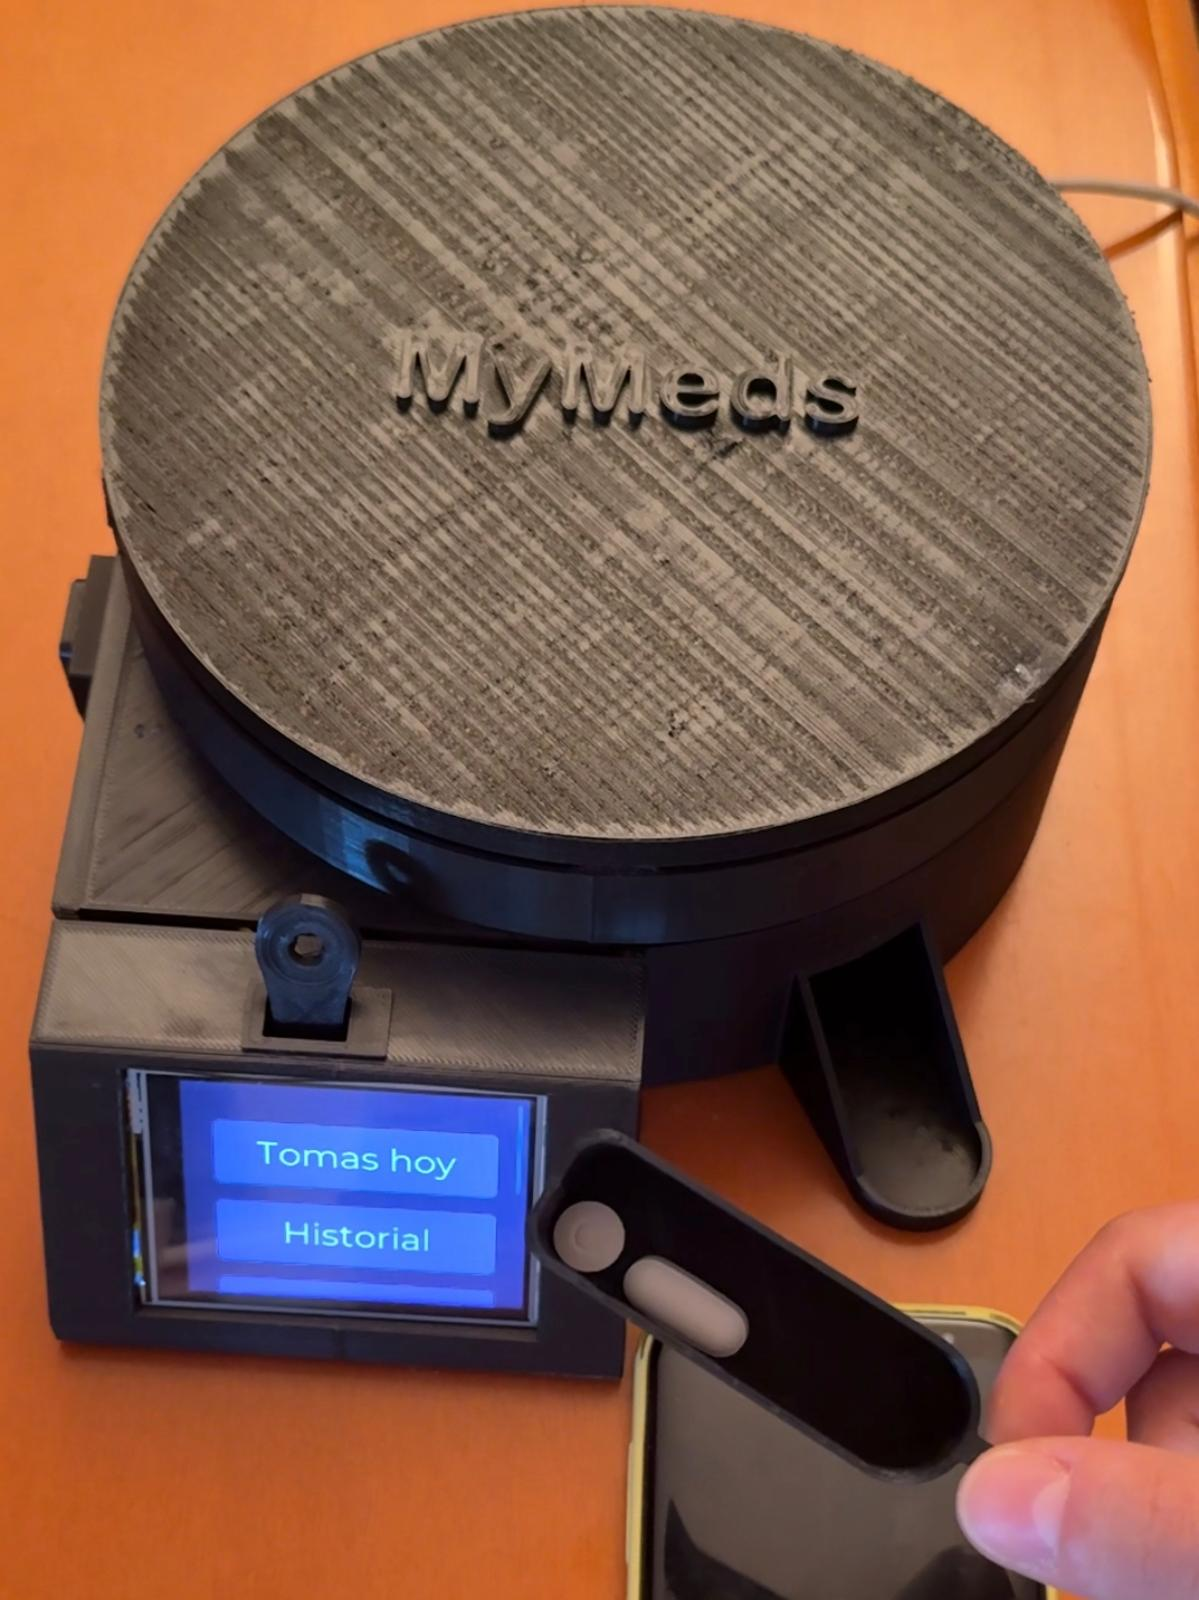
\includegraphics[width=0.5\linewidth]{figs/validacion.jpeg}
    \caption{Validación del proceso de dispensación.}
    \label{fig:validacion_disp}
\end{figure}

\section{Sincronización entre la aplicación móvil y el dispositivo}

La comunicación entre la aplicación móvil y el dispensador resulta esencial para mantener actualizada la configuración del sistema. Con el objetivo de verificar el correcto intercambio de información, se realizaron diferentes pruebas relacionadas con la sincronización de datos y el funcionamiento autónomo del dispositivo.\\

\subsection{Sincronización de tomas y configuración}

La correcta sincronización entre la aplicación móvil y el dispensador resulta fundamental para garantizar que la información utilizada por ambos sistemas sea coherente. Con el objetivo de validar esta funcionalidad, se realizaron diferentes pruebas destinadas a verificar el intercambio bidireccional de información relacionada con la configuración de las tomas programadas.\\

La validación de la sincronización se realizó mediante dos conjuntos de pruebas complementarios. En primer lugar, se verificó la correcta sincronización del catálogo de medicamentos entre la aplicación móvil y el dispositivo. Posteriormente, se evaluó la sincronización bidireccional de las tomas programadas, comprobando que las modificaciones realizadas desde cualquiera de las dos interfaces eran transmitidas correctamente al otro sistema. De esta forma se verificó que la configuración podía gestionarse indistintamente desde cualquiera de las dos interfaces sin generar inconsistencias ni conflictos entre los datos almacenados.\\

La Figura~\ref{fig:sync} muestra una captura correspondiente a ambas pruebas realizadas. El proceso de sincronización de medicamentos puede consultarse en el vídeo asociado\footnote{\url{https://tinyurl.com/uuppxkhh}}. Asimismo la sincronización bidireccional de tomas puede consultarse en el vídeo asociado\footnote{\url{https://tinyurl.com/yeyz9pc4}}.

\begin{figure}[H]
\centering
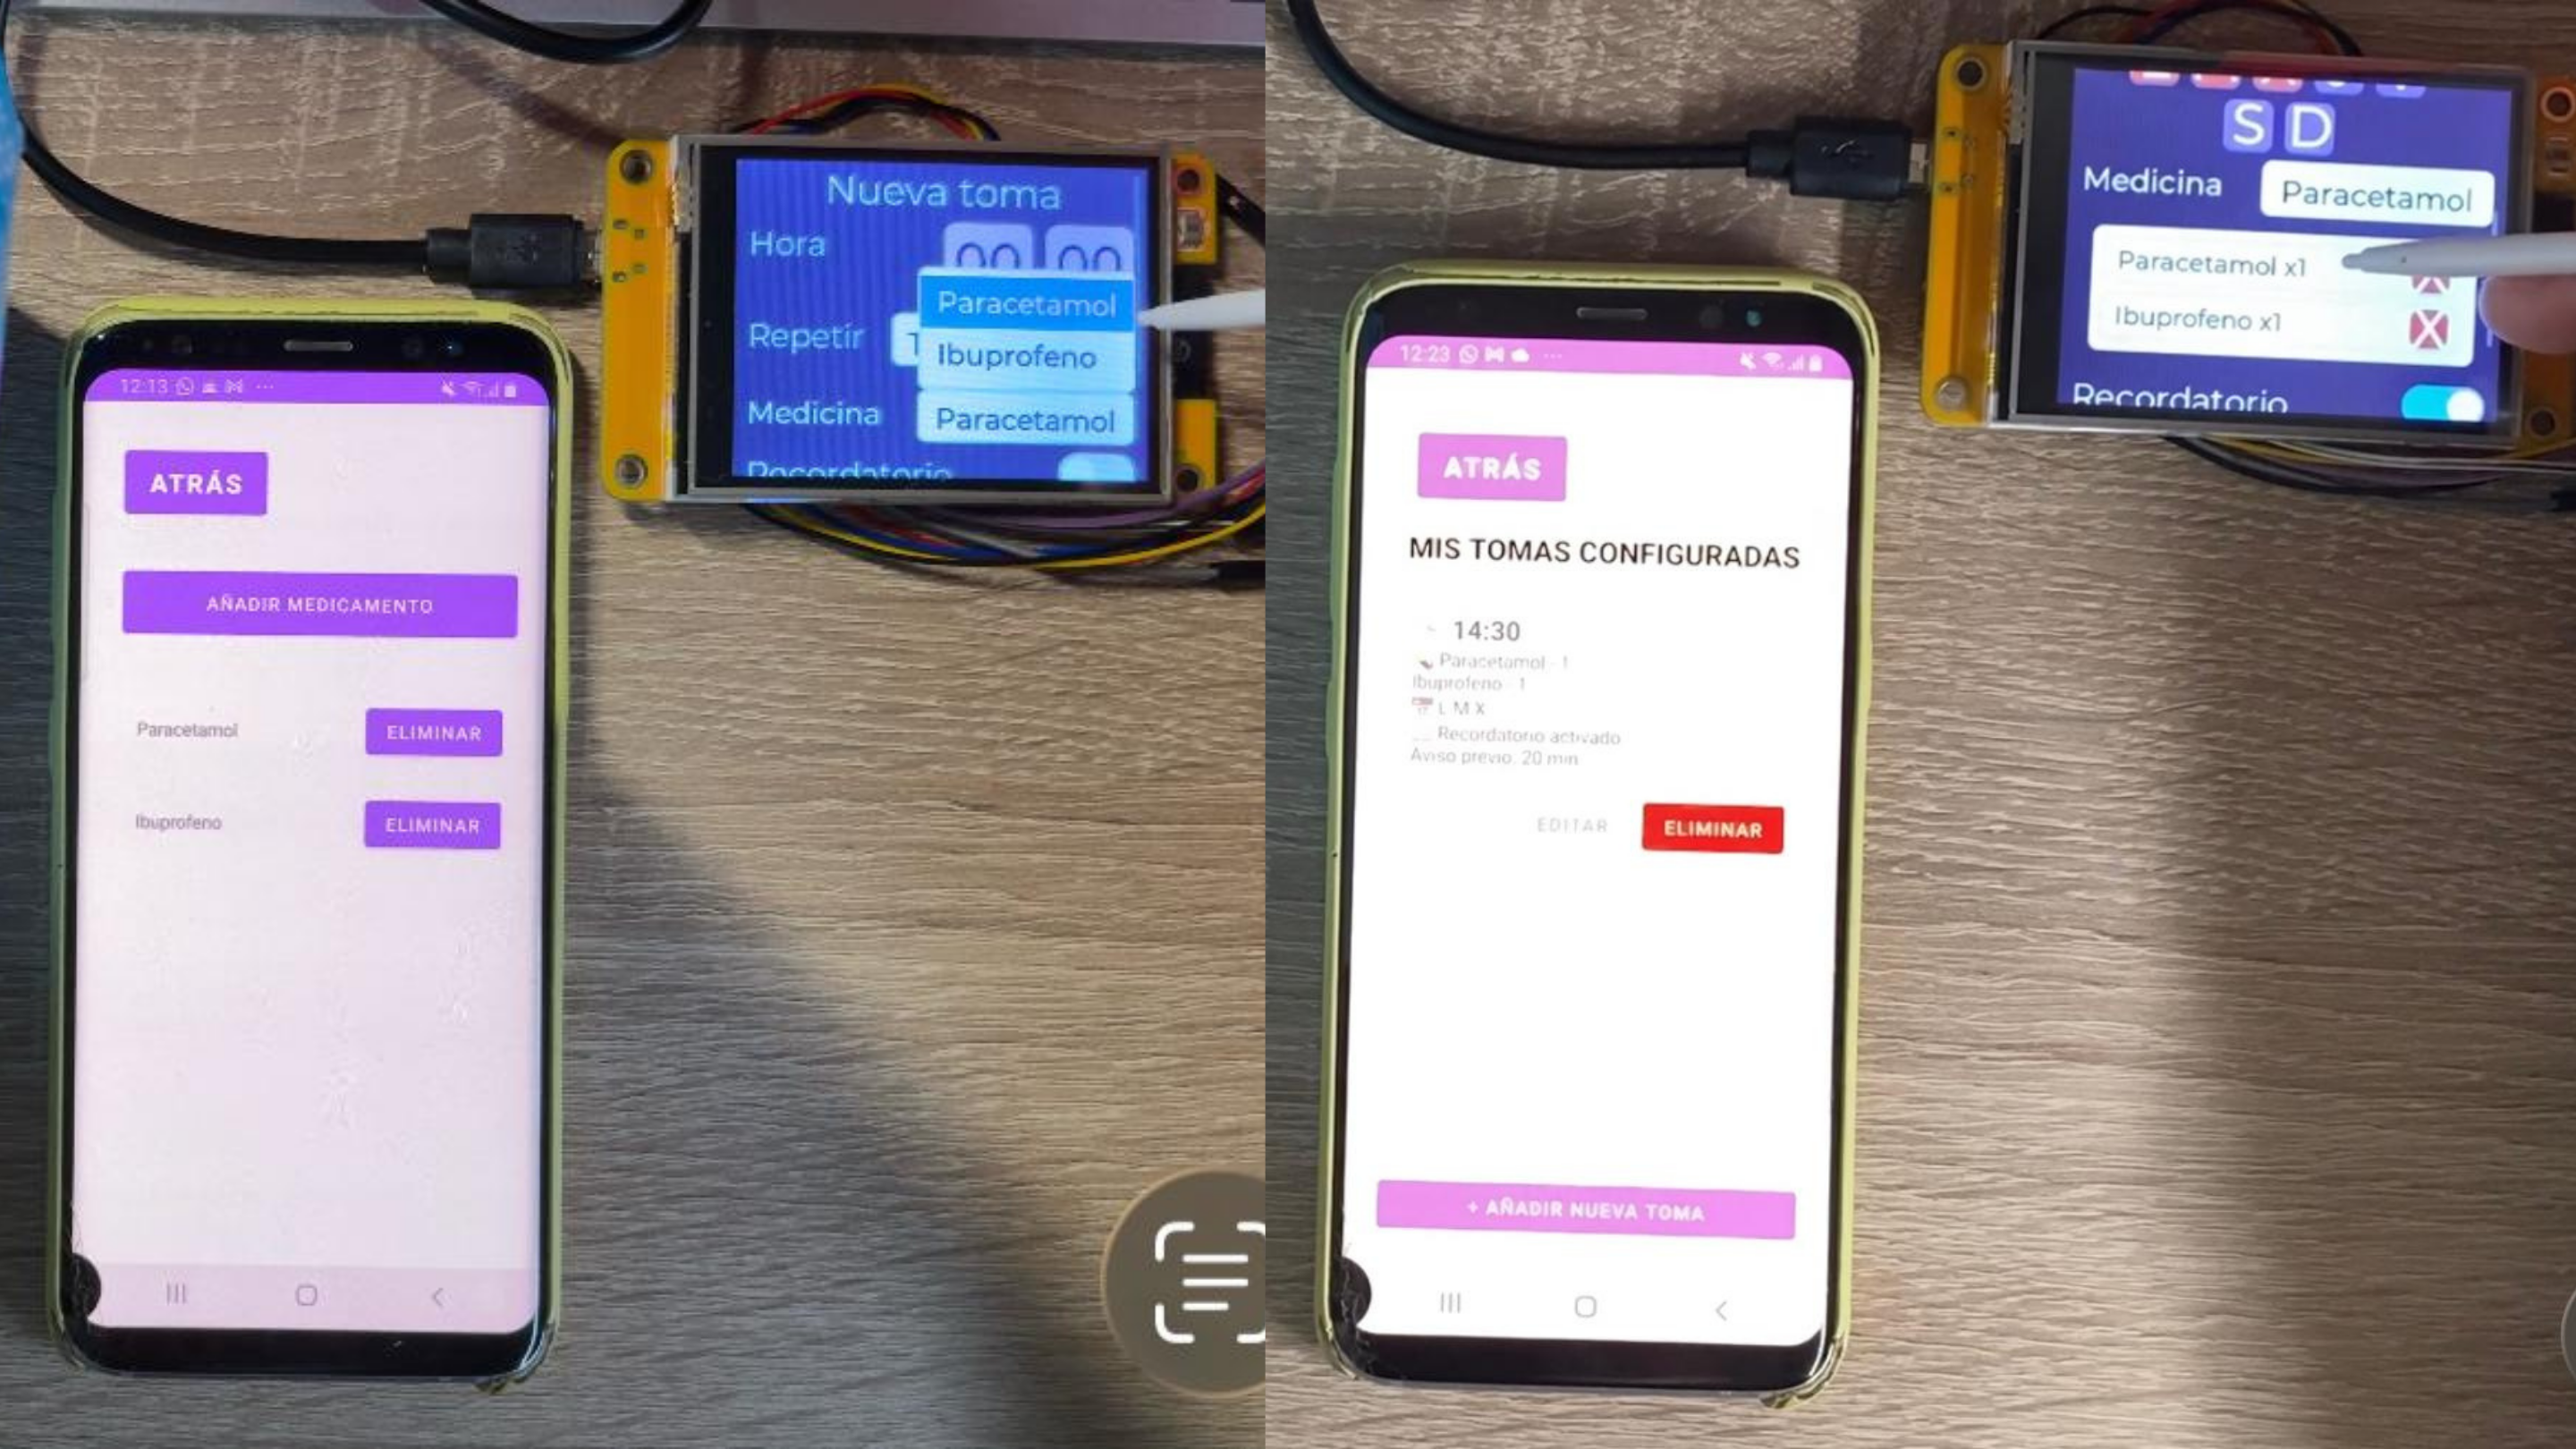
\includegraphics[width=0.85\textwidth]{figs/sincronizacion.png}
\caption{Validación de la sincronización de medicamentos y tomas entre la aplicación móvil y el dispositivo.}
\label{fig:sync}
\end{figure}

Los resultados obtenidos se resumen en la Tabla~\ref{tab:sincronizacion_tomas}.

\begin{table}[H]
\centering
\caption{Resultados de la validación de la sincronización bidireccional de tomas y configuración.}
\label{tab:sincronizacion_tomas}
\begin{tabular}{|l|c|}
\hline
\textbf{Prueba realizada} & \textbf{Resultado} \\ \hline
Creación de tomas desde Android & Correcto \\ \hline
Creación de tomas desde el dispositivo & Correcto \\ \hline
Modificación de tomas desde Android & Correcto \\ \hline
Modificación de tomas desde el dispositivo & Correcto \\ \hline
Eliminación de tomas desde Android & Correcto \\ \hline
Eliminación de tomas desde el dispositivo & Correcto \\ \hline
Consistencia de la configuración sincronizada & Correcto \\ \hline
\end{tabular}
\end{table}

Los ensayos realizados muestran que la sincronización bidireccional funciona correctamente, permitiendo gestionar la configuración desde cualquiera de los dos sistemas. Tras cada operación realizada, ambos componentes mantuvieron una representación idéntica de las tomas programadas, evitando inconsistencias y garantizando la coherencia de la información almacenada.

\subsection{Funcionamiento autónomo del dispositivo}

Una vez sincronizada la configuración, el dispensador debe ser capaz de funcionar de manera independiente sin requerir una conexión permanente con la aplicación móvil. Esta característica resulta esencial para garantizar la continuidad del servicio incluso cuando el dispositivo Android no se encuentra disponible.\\

La validación experimental se realizará con un ensayo en el que, tras sincronizar la configuración desde la aplicación móvil, se desconectará completamente el dispositivo Android y se verificará que el dispensador continúa ejecutando de forma autónoma las tareas programadas utilizando únicamente la información almacenada localmente.\\

La Figura~\ref{fig:func_autonomo} muestra una captura correspondiente a una de las pruebas realizadas. El desarrollo completo del experimento se puede consultar en el vídeo asociado\footnote{\url{https://tinyurl.com/3c78pjkb}}.

\begin{figure}[H]
\centering
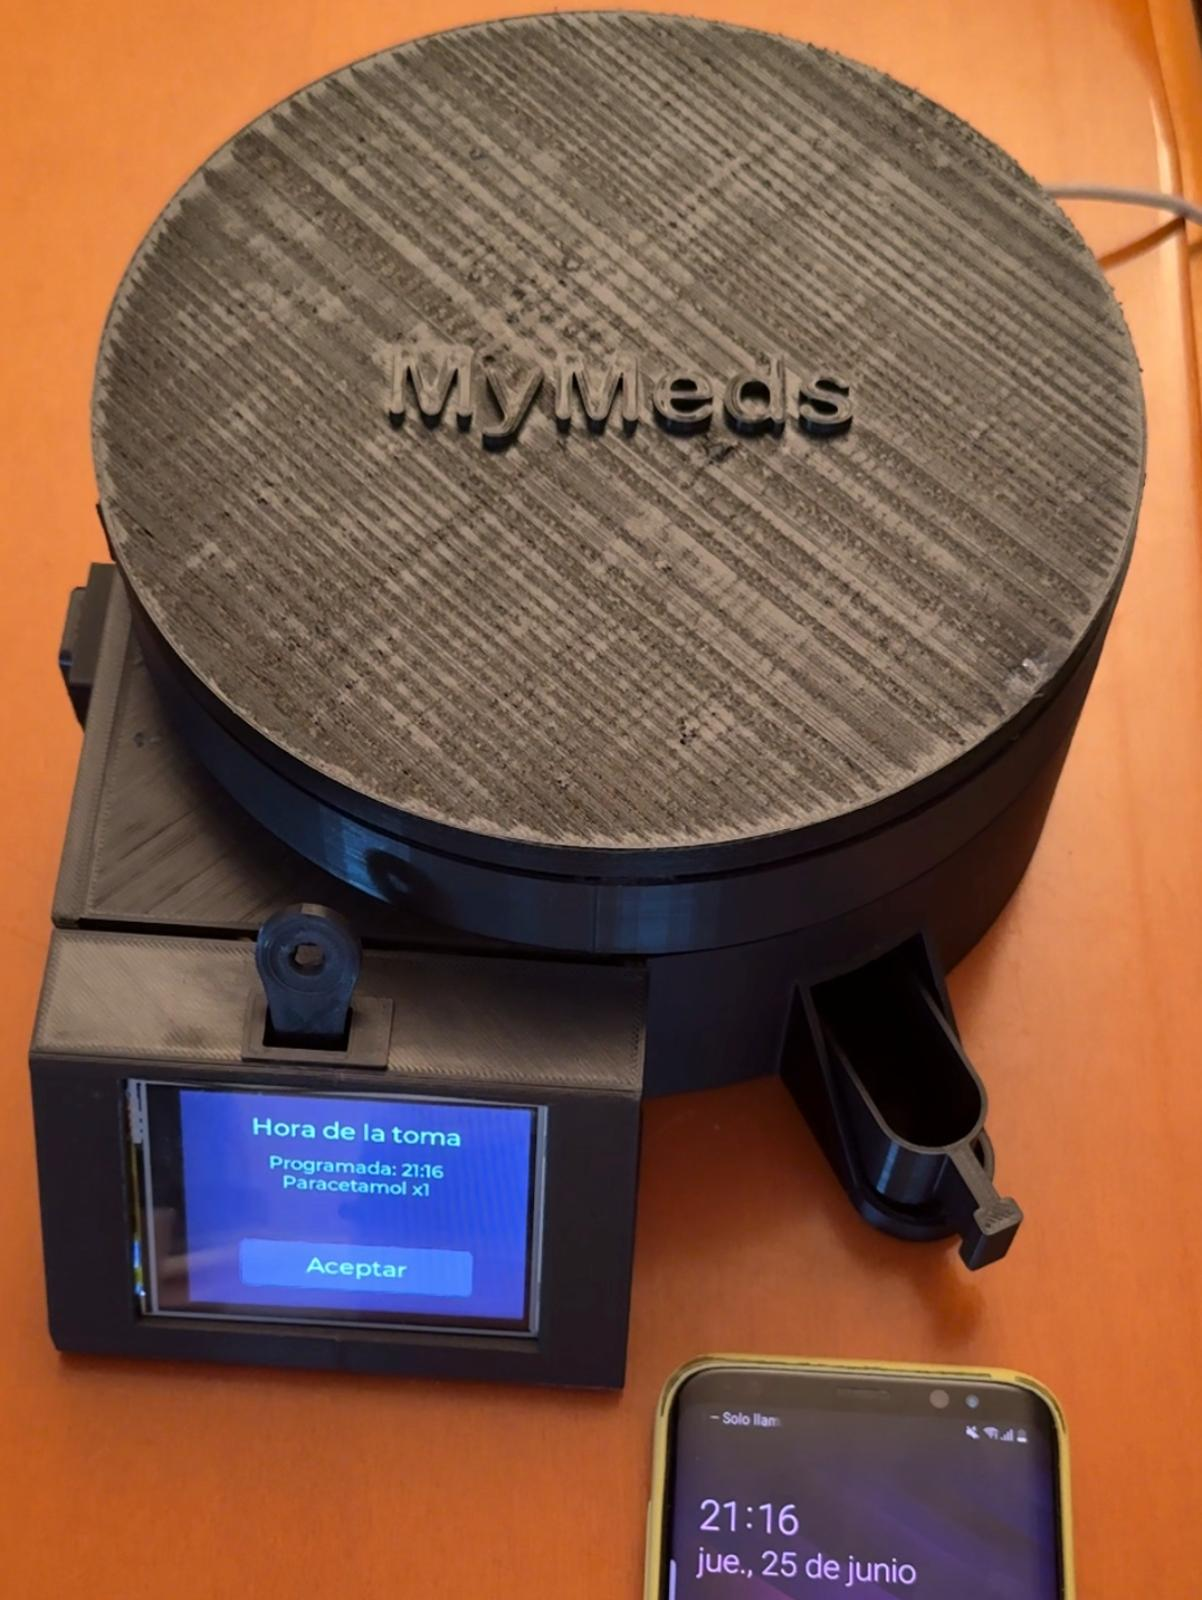
\includegraphics[width=0.5\textwidth]{figs/funcionamiento_autonomo.jpeg}
\caption{Funcionamiento autónomo del dispensador utilizando la configuración almacenada localmente.}
\label{fig:func_autonomo}
\end{figure}

Los resultados obtenidos se resume en la Tabla~\ref{tab:val_autonomo}.

\begin{table}[H]
\centering
\caption{Resultados de la validación del funcionamiento autónomo del dispositivo.}
\label{tab:val_autonomo}
\begin{tabular}{|l|c|}
\hline
\textbf{Prueba realizada} & \textbf{Resultado} \\ \hline
Funcionamiento sin conexión con Android & Correcto \\ \hline
Disponibilidad de las tomas programadas & Correcto \\ \hline
Activación de alarmas programadas & Correcto \\ \hline
Uso de la configuración almacenada & Correcto \\ \hline
\end{tabular}
\end{table}

\

Una vez completado el experimento, los resultados permitieron determinar el grado de autonomía alcanzado por el sistema y verificar que el dispensador puede continuar prestando sus funcionalidades esenciales sin depender de una conexión permanente con la aplicación móvil.

\section{Evaluación del pulsómetro}

El pulsómetro integrado constituye una de las funcionalidades complementarias incorporadas al dispositivo. Debido a la naturaleza de las señales biomédicas adquiridas y a la sensibilidad de este tipo de sensores a las condiciones de medida, se realizaron diferentes pruebas destinadas a evaluar la estabilidad, precisión y robustez en las mediciones.\\

\subsection{Estabilización de la medida}

Se consideró importante analizar el tiempo necesario para conseguir una medición estable de la frecuencia cardíaca antes de determinar la exactitud del pulsómetro integrado. El algoritmo implementado necesita acumular una cantidad mínima de latidos válidos antes de presentar al usuario una estimación, debido a las características de la señal fotopletismográfica obtenida por el sensor MAX30102.\\

Para medir este comportamiento, se llevaron a cabo cinco pruebas independientes en estado de reposo. En cada prueba, se anotó el tiempo que pasó desde que el dedo fue colocado sobre el sensor hasta que la primera lectura fue mostrada al usuario. También se registró el momento en que el buffer de medida llegó a su máxima capacidad y la lectura pudo ser considerada totalmente estabilizada. Los resultados obtenidos se muestran en la Tabla~\ref{tab:estabilizacion_pulso}.\\

\begin{table}[H]
\centering
\caption{Tiempo necesario para la obtención de una medición estable.}
\label{tab:estabilizacion_pulso}
\begin{tabular}{|c|c|c|}
\hline
\textbf{Ensayo} & \textbf{Primera lectura mostrada (s)} & \textbf{Buffer completo (s)} \\ \hline
1 & 17.17 & 23.27 \\ \hline
2 & 21.94 & 26.53 \\ \hline
3 & 18.69 & 23.24 \\ \hline
4 & 14.87 & 19.14 \\ \hline
5 & 12.58 & 17.25 \\ \hline
\textbf{Media} & \textbf{17.05} & \textbf{21.89} \\ \hline
\end{tabular}
\end{table}

Los resultados indican que el sistema necesita un promedio de 17.05 segundos para ofrecer al usuario la primera estimación de la frecuencia cardíaca y cerca de 21.89 segundos para finalizar el proceso de estabilización del parámetro.\\

Se registraron oscilaciones importantes en la señal adquirida durante los primeros segundos después de que se colocara el dedo. Este comportamiento es consecuencia de que el algoritmo requiere la detección de un número adecuado de latidos válidos para estimar una media representativa y la influencia del ruido presente en la señal fotopletismográfica. Cuando se llega a este umbral, la lectura tiende a estabilizarse progresivamente.
\begin{figure}[H]
    \centering
    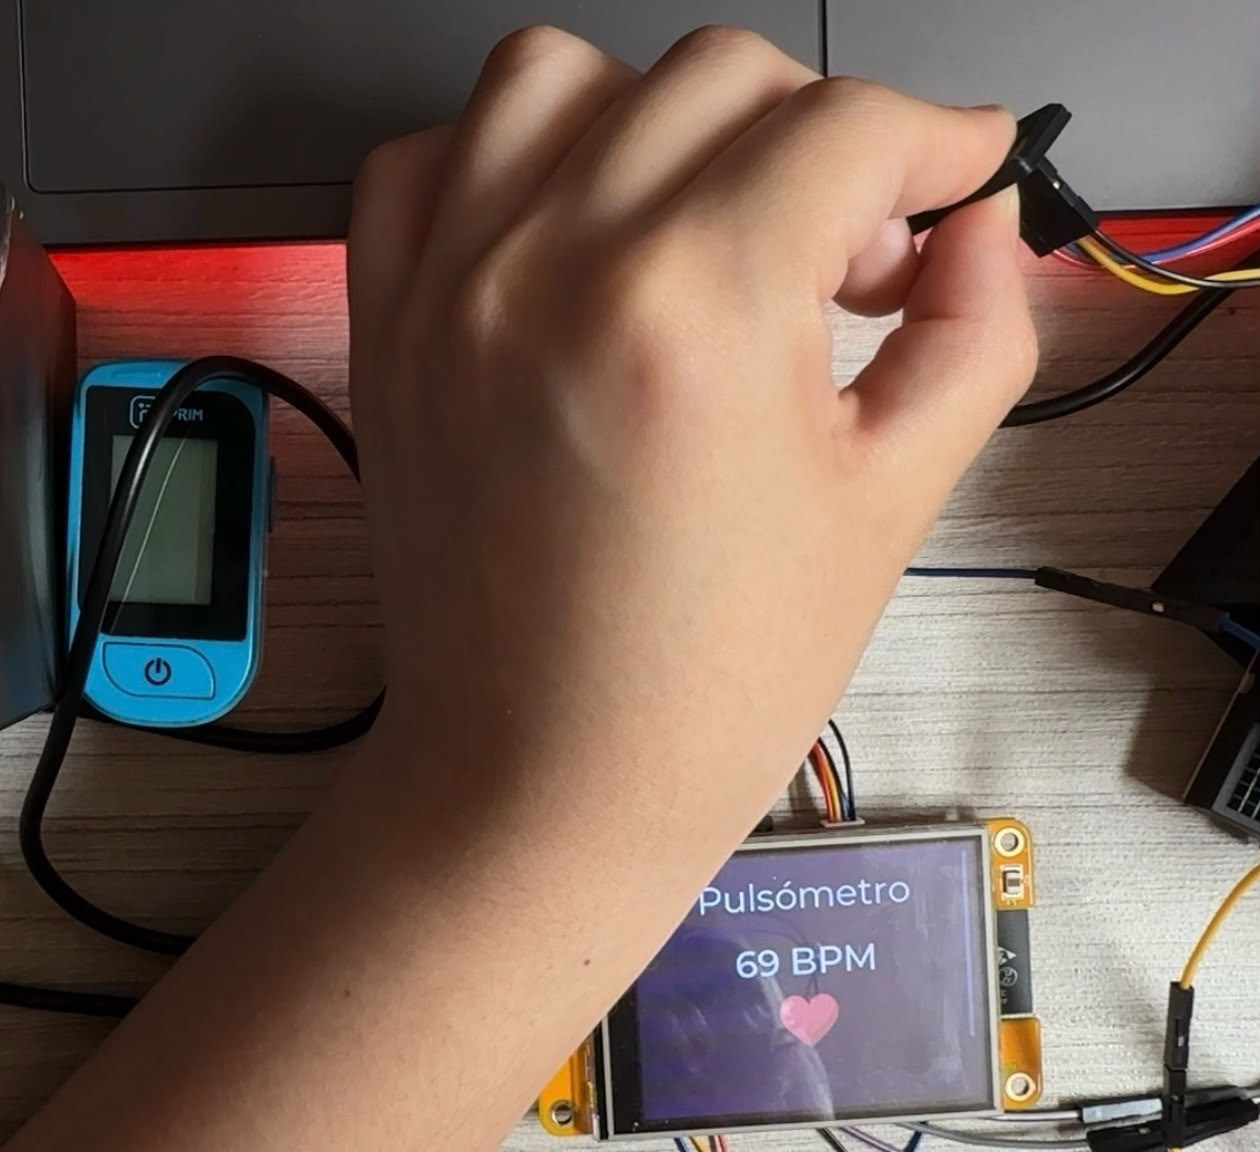
\includegraphics[width=0.55\textwidth]{figs/estabilizacion_medida.jpeg}
    \caption{Captura obtenida durante una de las pruebas de estabilización de la medida.}
    \label{fig:estabilizacion_medida}
\end{figure}

La Figura~\ref{fig:estabilizacion_medida} muestra una captura correspondiente a uno de los ensayos realizados. Con el fin de facilitar la reproducibilidad de los resultados obtenidos, el desarrollo completo de la prueba fue registrado en vídeo\footnote{\url{https://bit.ly/4oBEemg}}.\\

La diferencia que se ha notado entre los diferentes ensayos señala que el tiempo de estabilización depende de varios factores, incluyendo cómo está colocado el dedo, la calidad de la señal que capta el sensor, y las características fisiológicas del usuario. Este comportamiento impulsó la realización de pruebas adicionales para investigar cómo influyen las condiciones de medida, cuyos resultados se exponen en el siguiente apartado.\\

Por lo tanto, se puede concluir que el sistema desarrollado tiene la capacidad de ofrecer estimaciones estables de la frecuencia cardíaca, pero necesita un tiempo inicial para adquirir y procesar la señal antes de presentar una lectura confiable al usuario.

\subsection{Influencia de las condiciones de medida}

Después de analizar el proceso de estabilización de la medida, se estudió cómo la posición del dedo y la mano empleada afectan al comportamiento del pulsómetro. Como el sensor MAX30102 es óptico, la detección de latidos válidos y el tiempo requerido para conseguir una medición estable pueden verse alterados por factores como la presión que se ejerce sobre él, la calidad del contacto o la dirección del dedo.\\

Para evaluar este comportamiento se realizaron dos rondas de pruebas utilizando cuatro configuraciones distintas: mano izquierda en orientación vertical, mano izquierda en orientación horizontal, mano derecha en orientación vertical y mano derecha en orientación horizontal. En cada ensayo se registró el tiempo transcurrido hasta la aparición de la primera lectura mostrada al usuario y el tiempo necesario para completar el buffer de medida.\\

La Figura~\ref{fig:posiciones_pulso} muestra las diferentes configuraciones evaluadas durante las pruebas. Para que los resultados sean más fáciles de reproducir, se grabaron las dos rondas completas de ensayos\footnote{Vídeo correspondiente a la primera ronda de pruebas: \url{https://bit.ly/4uuQOVv}}\footnote{Vídeo correspondiente a la segunda ronda de pruebas: \url{https://tinyurl.com/2c2ae7fa}}.

\begin{figure}[H]
\centering
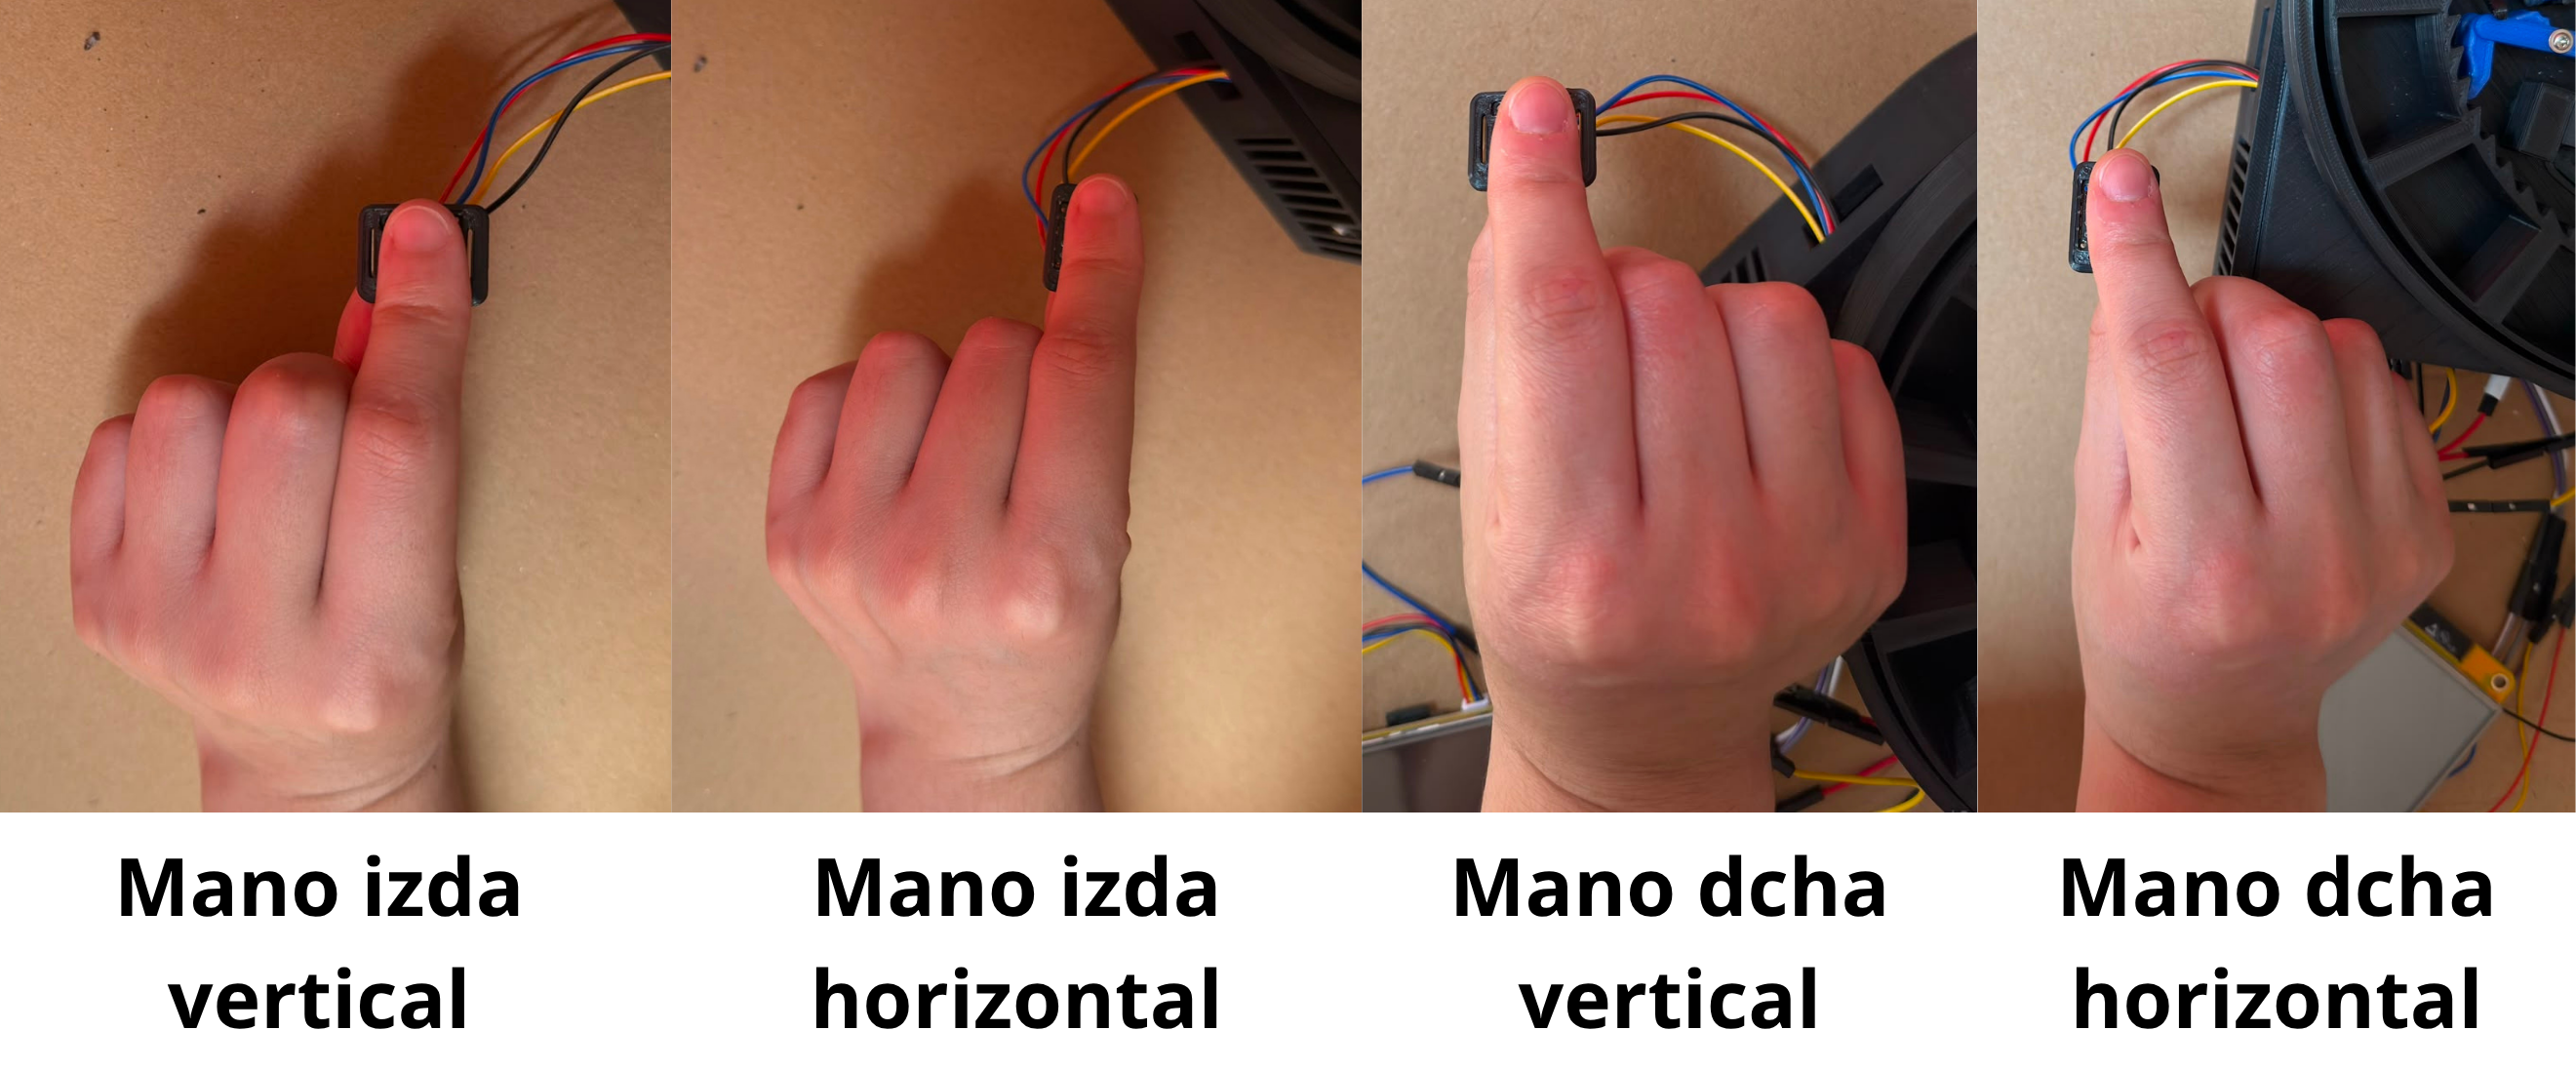
\includegraphics[width=\textwidth]{figs/posiciones_pulso.png}
\caption{Posiciones utilizadas durante las pruebas de influencia de las condiciones de medida.}
\label{fig:posiciones_pulso}
\end{figure}

Los resultados obtenidos en la primera ronda de ensayos se muestran en la Tabla~\ref{tab:pulso_ronda1}.

\begin{table}[H]
\centering
\caption{Resultados obtenidos durante la primera ronda de pruebas.}
\label{tab:pulso_ronda1}
\begin{tabular}{|l|c|c|}
\hline
\textbf{Configuración} & \textbf{Primera lectura (s)} & \textbf{Buffer completo (s)} \\ \hline
Mano izquierda vertical & 41.12 & 49.12 \\ \hline
Mano izquierda horizontal & 26.73 & 34.77 \\ \hline
Mano derecha vertical & 16.92 & 21.46 \\ \hline
Mano derecha horizontal & 35.05 & 42.89 \\ \hline
\end{tabular}
\end{table}

La segunda ronda de ensayos se realizó con el mismo procedimiento, obteniéndose los resultados mostrados en la Tabla~\ref{tab:pulso_ronda2}.

\begin{table}[H]
\centering
\caption{Resultados obtenidos durante la segunda ronda de pruebas.}
\label{tab:pulso_ronda2}
\begin{tabular}{|l|c|c|}
\hline
\textbf{Configuración} & \textbf{Primera lectura (s)} & \textbf{Buffer completo (s)} \\ \hline
Mano izquierda vertical & 17.24 & 22.19 \\ \hline
Mano izquierda horizontal & 33.76 & 38.26 \\ \hline
Mano derecha vertical & 12.66 & 19.29 \\ \hline
Mano derecha horizontal & 21.39 & 32.92 \\ \hline
\end{tabular}
\end{table}

A partir de los resultados obtenidos tras las dos rondas se calcularon los tiempos medios obtenidos para cada configuración, cuyos resultados se recogen en la Tabla~\ref{tab:condiciones_medida}.

\begin{table}[H]
\centering
\caption{Tiempos medios obtenidos para cada configuración evaluada.}
\label{tab:condiciones_medida}
\begin{tabular}{|l|c|c|}
\hline
\textbf{Configuración} & \textbf{Primera lectura $\bar{x}$ (s)} & \textbf{Buffer completo $\bar{x}$ (s)} \\ \hline
Mano izquierda vertical & 29.18 & 35.66 \\ \hline
Mano izquierda horizontal & 30.25 & 36.52 \\ \hline
Mano derecha vertical & 14.79 & 20.38 \\ \hline
Mano derecha horizontal & 28.22 & 37.91 \\ \hline
\end{tabular}
\end{table}

Los resultados que se han conseguido demuestran que el tiempo necesario para conseguir una lectura estable está significativamente influenciado por las condiciones de medición. En las configuraciones analizadas, la que corresponde a la mano derecha en orientación vertical mostró de manera consistente los tiempos más cortos, tanto para la primera lectura como para la estabilización completa de la medida.\\

Por el contrario, las configuraciones restantes mostraron tiempos superiores y una mayor variabilidad entre ensayos. Estas diferencias pueden deberse a variaciones en la calidad de la señal fotopletismográfica captada por el sensor, producidas por cambios en la posición del dedo, la distribución del flujo sanguíneo o el grado de contacto entre la piel y los elementos ópticos del MAX30102.\\

Sin embargo, a pesar de que las condiciones de medición afectaron en el tiempo necesario para obtener una lectura estable, el sistema logró ofrecer en todos los casos un cálculo preciso de la frecuencia cardíaca. En consecuencia, se puede determinar que el pulsómetro integrado tiene un rendimiento sólido ante diversas maneras de uso. Sin embargo, durante las pruebas realizadas, la colocación vertical del dedo sobre la mano derecha ofreció los resultados más óptimos.


\subsection{Comparación con dispositivos de referencia}

Se contrastaron los resultados conseguidos con los que proporcionó un pulsioxímetro comercial de dedo, que fue empleado como aparato de referencia con la finalidad de analizar la exactitud de las mediciones ejecutadas por el pulsómetro integrado. Se llevaron a cabo todas las mediciones en condiciones de reposo y empleando la mano izquierda en vertical. Para cada ensayo se registró la frecuencia cardíaca indicada por ambos dispositivos una vez que las mediciones alcanzaron un estado estable. Los resultados obtenidos se muestran en la Tabla~\ref{tab}.\\

\begin{table}[H]
\centering
\caption{Comparación entre mediciones de \textit{MyMeds} y el pulsioxímetro comercial.}
\label{tab}
\begin{tabular}{|c|c|c|c|}
\hline
\textbf{Ensayo} & \textbf{MyMeds (BPM)} & \textbf{Pulsioxímetro (BPM)} & \textbf{Error absoluto (BPM)} \\ \hline
1 & 65 & 66 & 1 \\ \hline
2 & 62 & 65 & 3 \\ \hline
3 & 73 & 74 & 1 \\ \hline
4 & 70 & 74 & 4 \\ \hline
$\bar{x}$ & 67.5 & 69.75 & 2.25 \\ \hline
\end{tabular}
\end{table}

\

Los resultados logrados muestran una concordancia notable entre las mediciones efectuadas por \textit{MyMeds} y las proporcionadas por el pulsioxímetro de referencia. En tres de los cuatro ensayos llevados a cabo se encontró una diferencia igual o menor a 3 BPM con un error medio absoluto de 2.25 BPM. Se registró un error máximo de 4 BPM.\\

La Figura~\ref{fig:comparacion} muestra una captura obtenida durante una de las pruebas de comparación realizadas. El desarrollo completo de los cuatro ensayos puede consultarse en el vídeo asociado\footnote{\url{https://tinyurl.com/3ezx7aew}}.

\begin{figure}[H]
\centering
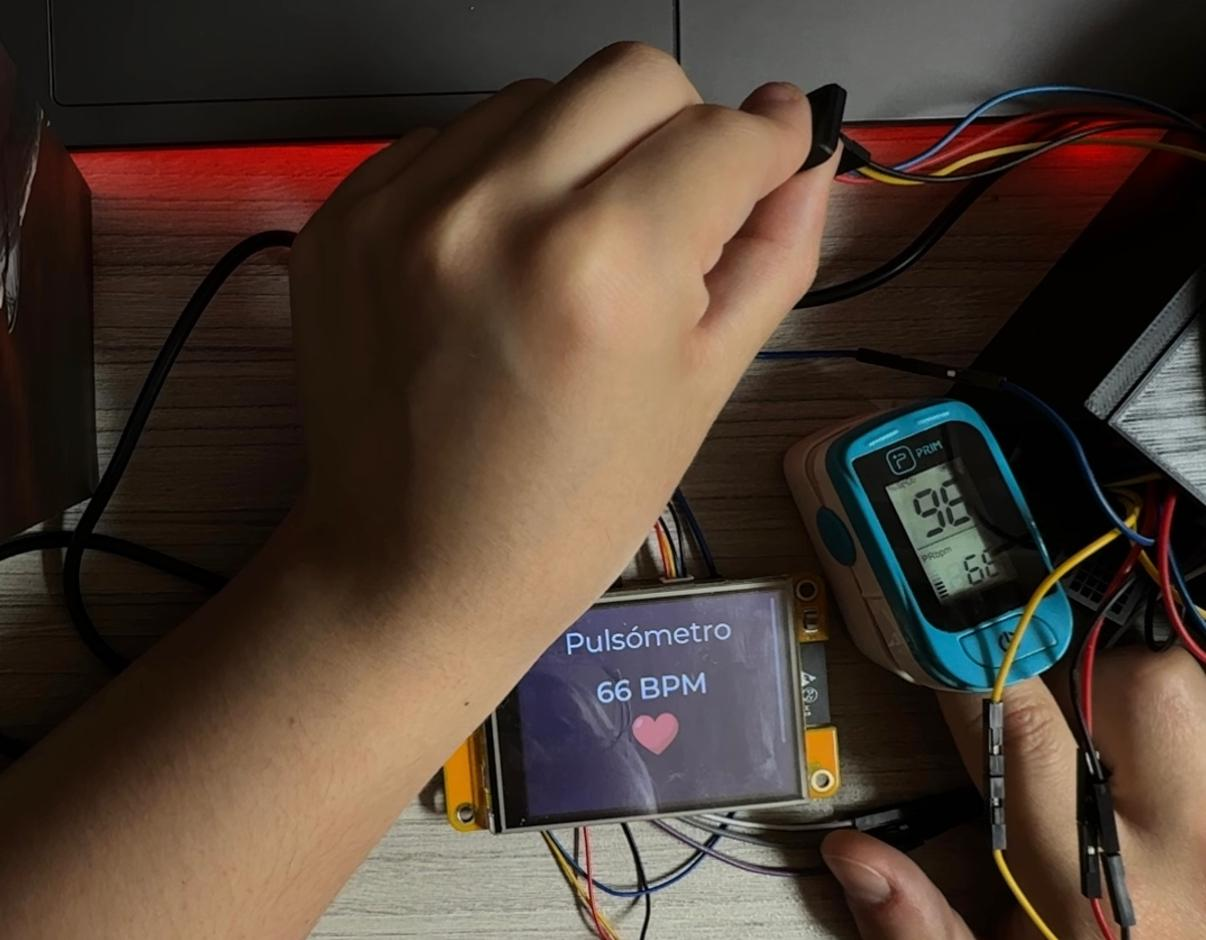
\includegraphics[width=0.65\textwidth]{figs/comparacion_pulsometro.jpeg}
\caption{Comparación entre MyMeds y el pulsioxímetro comercial durante una de las pruebas realizadas.}
\label{fig:comparacion}
\end{figure}

Las diferencias que se han observado pueden deberse a múltiples motivos, como el ruido en la señal fotopletismográfica, las fluctuaciones fisiológicas naturales que ocurren entre mediciones sucesivas, y las discrepancias entre los algoritmos de procesamiento empleados por cada uno de los dispositivos.\\

Además, los ensayos mostraron que ambos sistemas se comportaban dinámicamente de manera diferente. El pulsioxímetro comercial respondía de manera casi instantánea a alteraciones importantes en la frecuencia cardíaca, mientras que \textit{MyMeds} modificaba el valor presentado de un modo más gradual.\\

Como consecuencia, \textit{MyMeds} muestra una estabilidad más alta en las lecturas mostradas, aunque a costa de un tiempo de respuesta un poco más largo cuando ocurren cambios rápidos en la frecuencia cardíaca. Sin embargo, los resultados obtenidos muestran que el sistema desarrollado ofrece estimaciones que se aproximan adecuadamente a las de un dispositivo comercial, lo cual valida su uso como herramienta de monitoreo orientativa en el marco del proyecto.\\

\

\

\section{Persistencia y almacenamiento de datos}

Además de las funcionalidades de dispensación y monitorización biomédica, el sistema incorpora mecanismos de almacenamiento persistente que permiten conservar tanto la configuración del dispositivo como el histórico de mediciones realizadas. Con el fin de validar estos mecanismos, se llevaron a cabo diferentes pruebas relacionadas con la conservación y recuperación de la información almacenada.\\

\subsection{Conservación de la configuración}

Además del almacenamiento del historial de mediciones, el sistema desarrollado incorpora mecanismos de persistencia destinados a conservar la configuración del dispositivo entre reinicios. Con el fin de validar su correcto funcionamiento, se realizaron diferentes pruebas orientadas a comprobar la conservación de las tomas programadas y del PIN de acceso tras apagar y volver a encender el dispositivo.\\

En una primera prueba se configuraron varias tomas de medicación utilizando la aplicación móvil y posteriormente se reinició completamente el sistema. Tras el arranque, se verificó que la información asociada a las tomas programadas seguía disponible y podía consultarse desde el dispositivo sin necesidad de realizar una nueva sincronización. Igualmente, al modificar dichas tomas o eliminar alguna, seguían disponibles pero actualizadas. La Figura~\ref{fig:persistencia_tomas} muestra una captura correspondiente a esta prueba. El desarrollo completo del ensayo puede consultarse en el vídeo asociado\footnote{\url{https://tinyurl.com/uuppxkhh}}.

\begin{figure}[H]
\centering
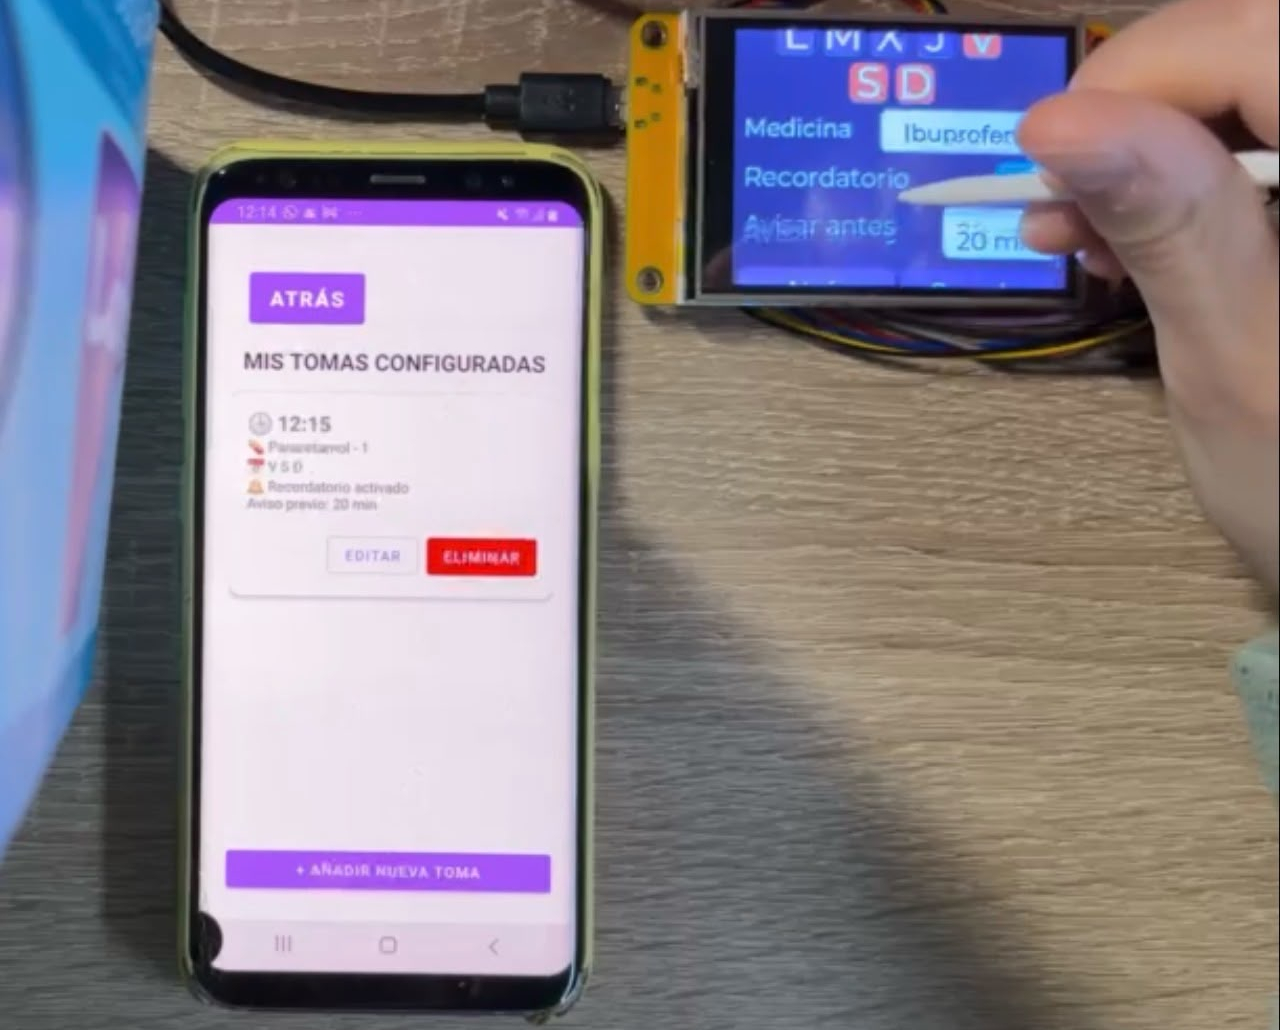
\includegraphics[width=0.45\textwidth]{figs/persistencia_tomas.jpeg}
\caption{Validación de la conservación de las tomas programadas tras reiniciar el dispositivo.}
\label{fig:persistencia_tomas}
\end{figure}

Posteriormente se realizó una segunda prueba destinada a verificar la persistencia del PIN de acceso. Para ello se configuró un PIN personalizado, se apagó completamente el dispositivo y se volvió a encender. Tras el reinicio, se comprobó que el sistema continuaba solicitando el mismo PIN configurado previamente. Además, se verificó que tras modificar el PIN en cualquiera de los dos dispositivos, el PIN se actualizaba en ambos y persistía de igual manera. La Figura~\ref{fig:persistencia_pin} muestra una captura correspondiente a esta validación. El vídeo completo de la prueba puede consultarse en línea\footnote{\url{https://tinyurl.com/t79yyy9z}}.

\begin{figure}[H]
\centering
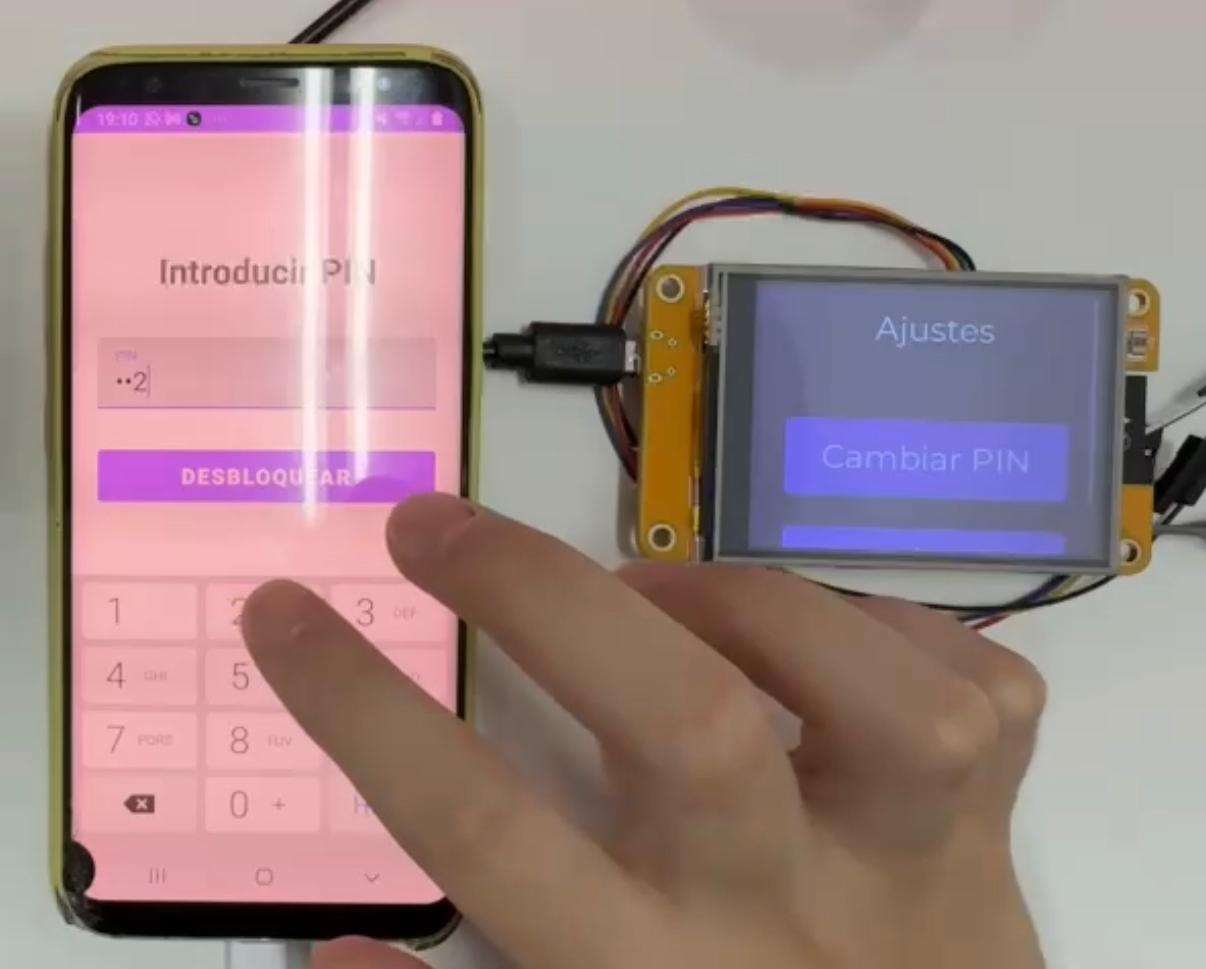
\includegraphics[width=0.6\textwidth]{figs/persistencia_pin.jpeg}
\caption{Validación de la conservación del PIN de acceso tras reiniciar el dispositivo.}
\label{fig:persistencia_pin}
\end{figure}

Los resultados obtenidos se resumen en la Tabla~\ref{tab:persistencia_configuracion}.

\begin{table}[H]
\centering
\caption{Validación de la persistencia de la configuración del sistema.}
\label{tab:persistencia_configuracion}
\begin{tabular}{|l|c|}
\hline
\textbf{Elemento evaluado} & \textbf{Resultado} \\ \hline
Tomas programadas conservadas tras reinicio & Correcto \\ \hline
PIN conservado tras reinicio & Correcto \\ \hline
Necesidad de reconfiguración manual & No \\ \hline
\end{tabular}
\end{table}

Los resultados obtenidos muestran que la información de configuración permanece almacenada correctamente tras el
apagado y encendido del dispositivo. Esto confirma el correcto funcionamiento de los mecanismos de almacenamiento persistente implementados, permitiendo que el usuario conserve la configuración del sistema sin necesidad de repetir el proceso de configuración tras cada reinicio.

\subsection{Almacenamiento del historial de mediciones}

Además de mostrar la frecuencia cardíaca en tiempo real, el sistema desarrollado incorpora un mecanismo de almacenamiento persistente que permite conservar un historial de las mediciones realizadas por el usuario. Con el fin de validar su correcto funcionamiento, se llevaron a cabo diferentes pruebas destinadas a verificar el almacenamiento de los datos en la tarjeta microSD que incorpora el dispositivo, su posterior recuperación desde este, y su sincronización con la aplicación móvil.\\

Durante las pruebas se realizaron varias mediciones de frecuencia cardíaca que fueron almacenadas automáticamente en un fichero CSV alojado en la tarjeta SD. La Figura~\ref{fig:csv} muestra una captura del archivo utilizado para almacenar el historial de mediciones.

\begin{figure}[H]
\centering
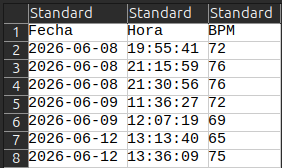
\includegraphics[width=0.5\textwidth]{figs/historial_csv.png}
\caption{Archivo CSV utilizado para almacenar el historial de pulsaciones.}
\label{fig:csv}
\end{figure}

Posteriormente se verificó que las mediciones almacenadas podían recuperarse correctamente desde la interfaz del dispositivo. La Figura~\ref{fig:historial_esp} muestra la pantalla de historial implementada en el ESP32, donde se visualizan las últimas 10 mediciones registradas.

\begin{figure}[H]
\centering
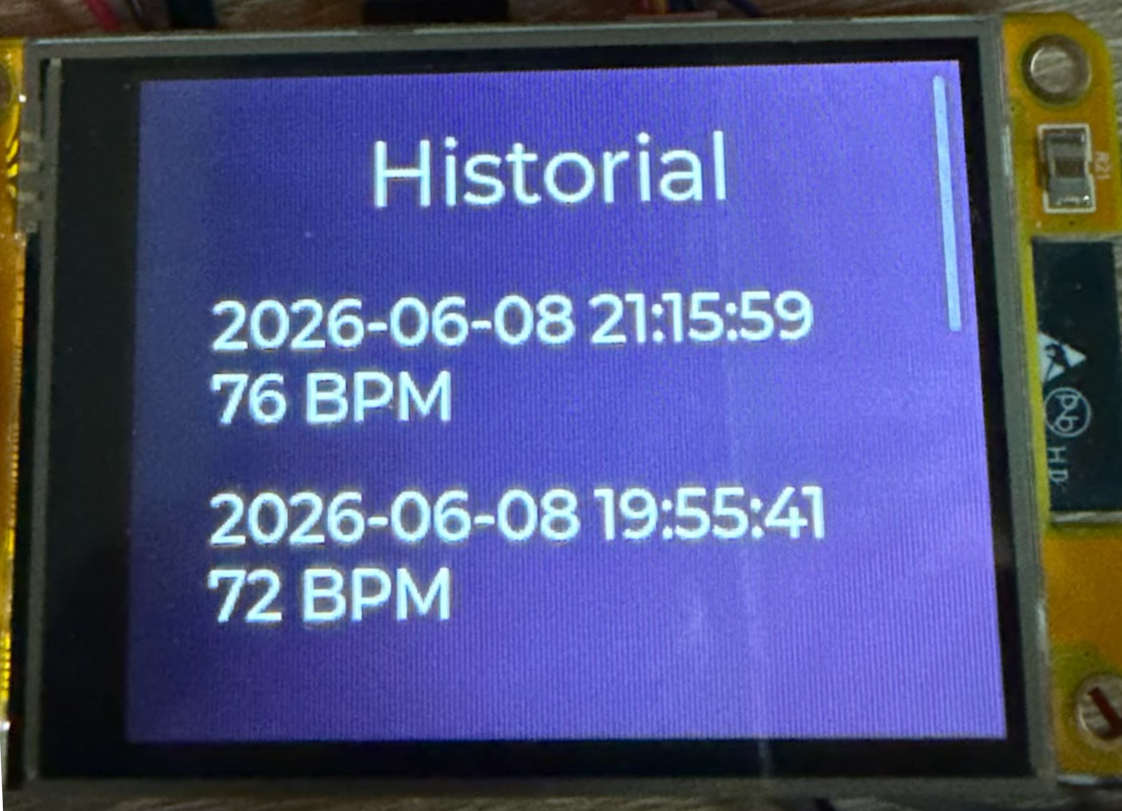
\includegraphics[width=0.45\textwidth]{figs/historial_esp.jpeg}
\caption{Visualización del historial de pulsaciones desde el dispositivo.}
\label{fig:historial_esp}
\end{figure}

Una vez comprobada la recuperación local de los datos, se validó la sincronización con la aplicación móvil mediante la API REST implementada. La Figura~\ref{fig:historial_app} muestra el historial descargado desde la aplicación Android, incluyendo la representación gráfica de las mediciones almacenadas.

\begin{figure}[H]
\centering
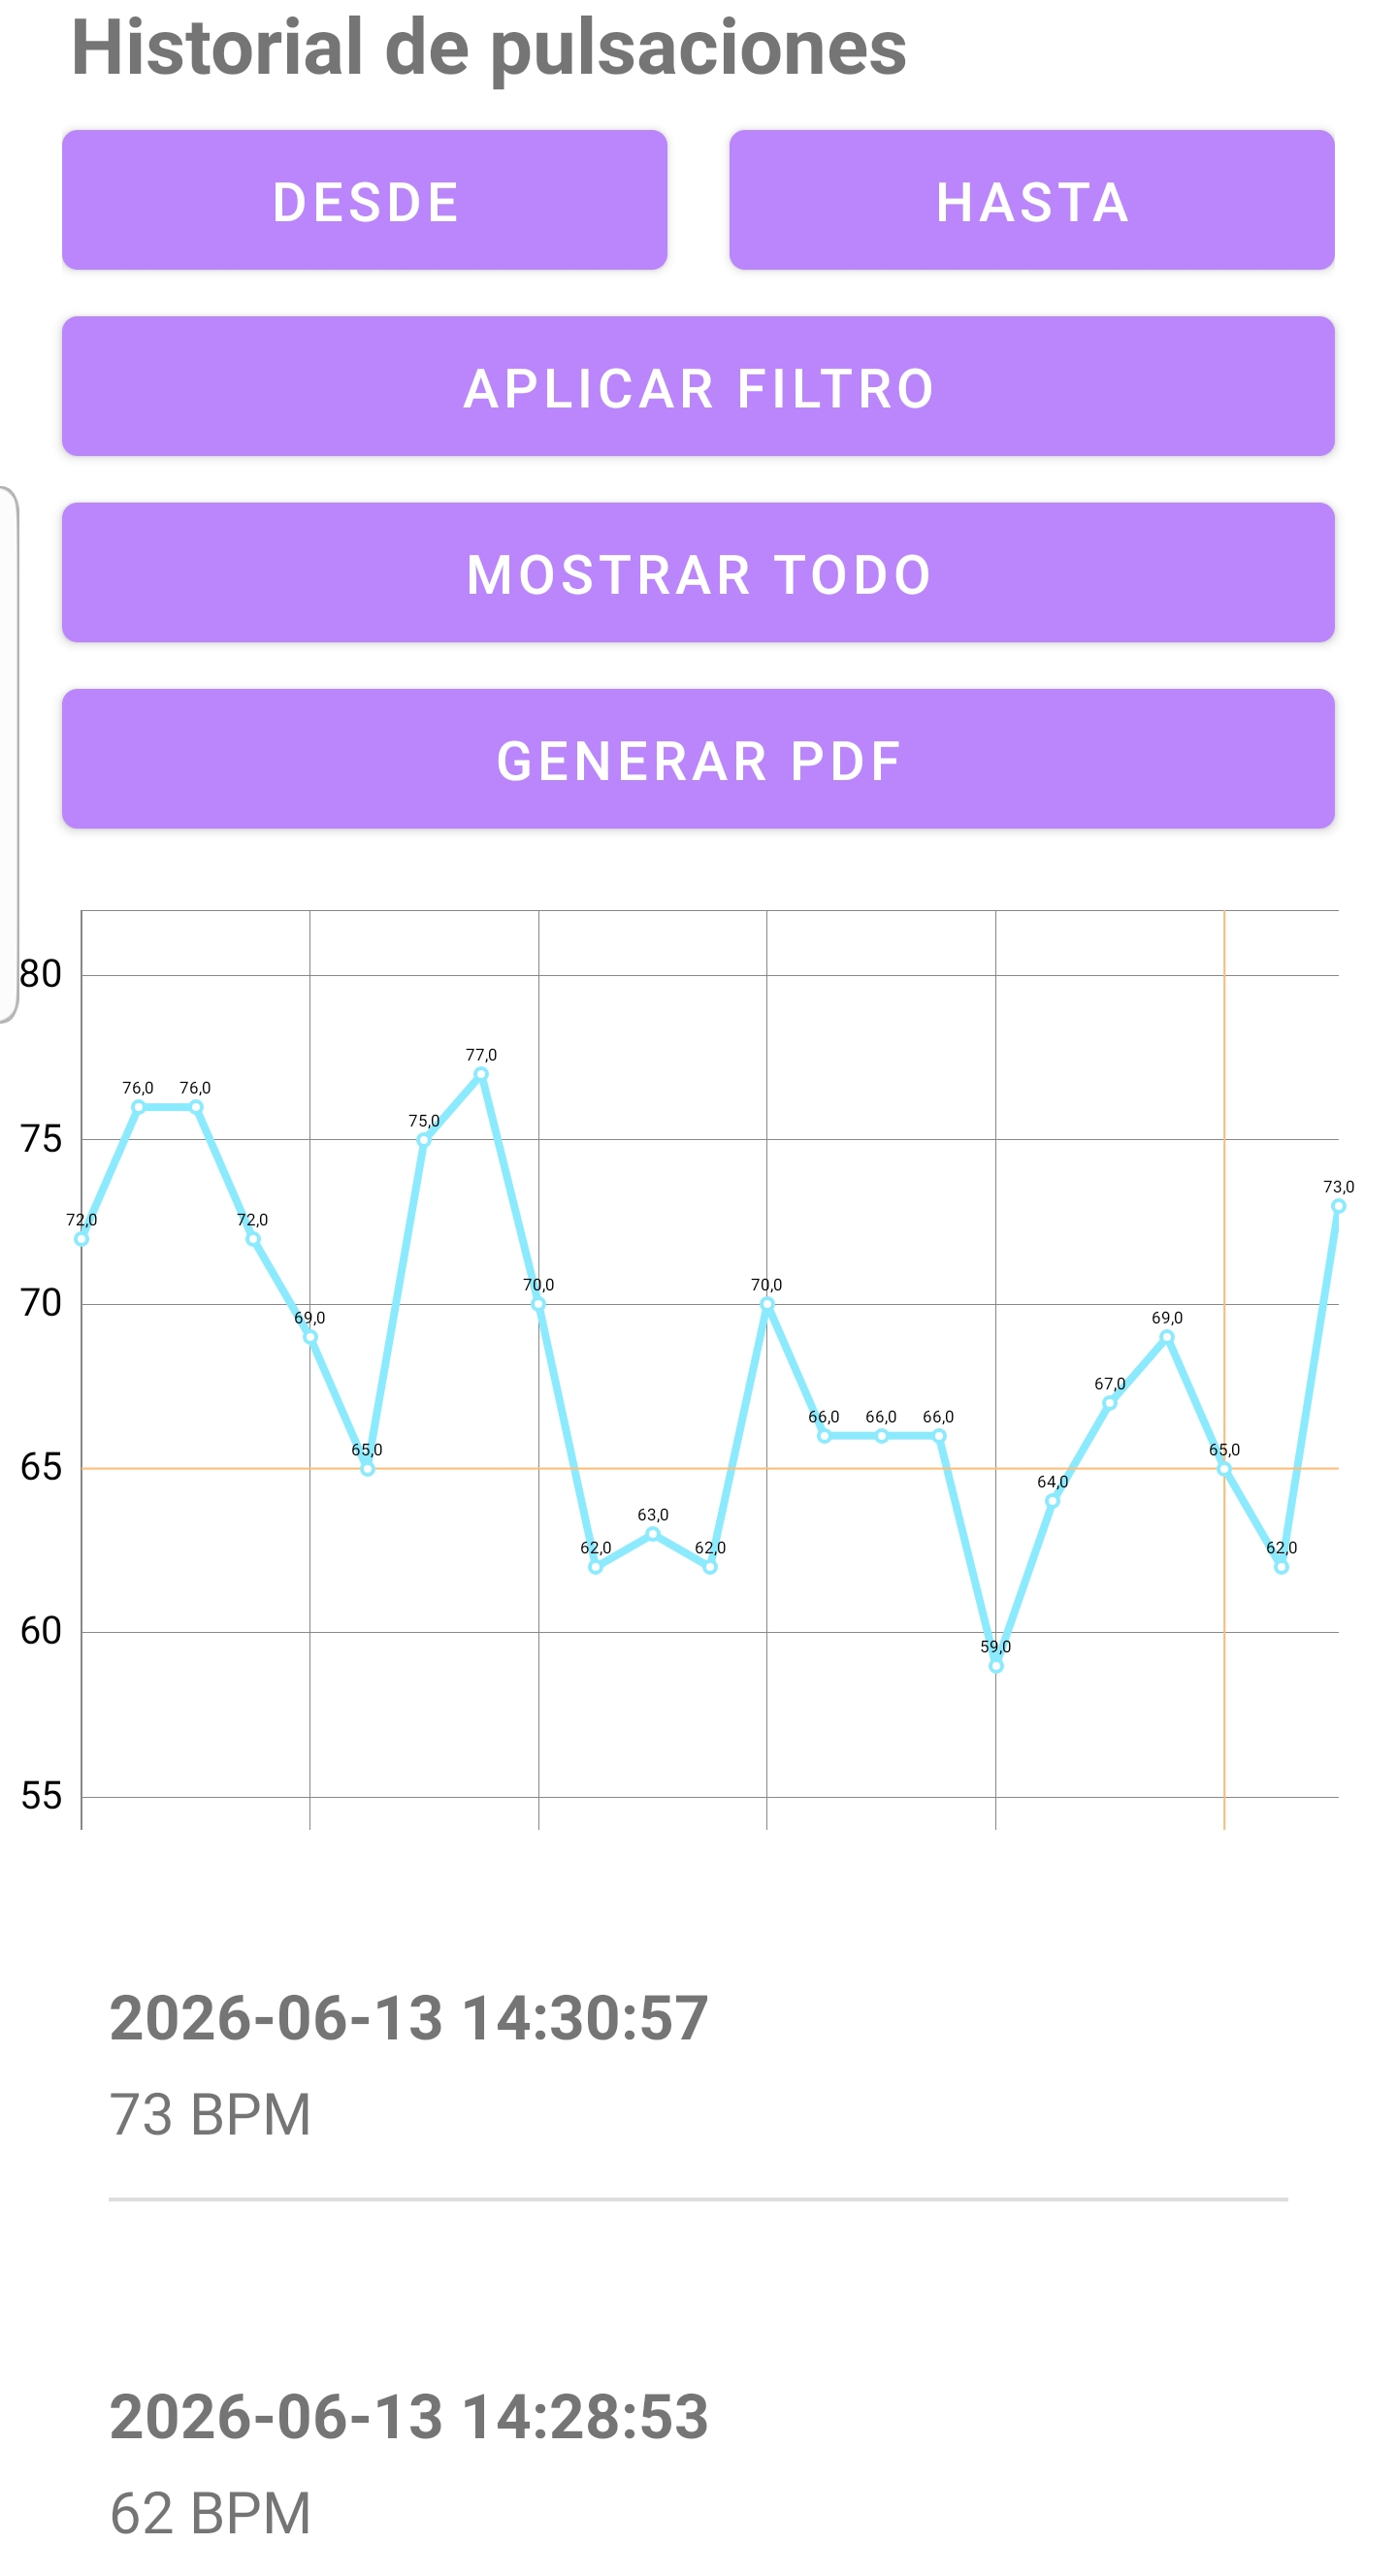
\includegraphics[width=0.3\textwidth]{figs/historial_android.jpg}
\caption{Historial de pulsaciones recuperado desde la aplicación móvil.}
\label{fig:historial_app}
\end{figure}

Finalmente, se verificó la correcta generación de informes PDF a partir de los datos recuperados. La Figura~\ref{fig:pdf} muestra un ejemplo del documento generado por la aplicación.

\begin{figure}[H]
\centering
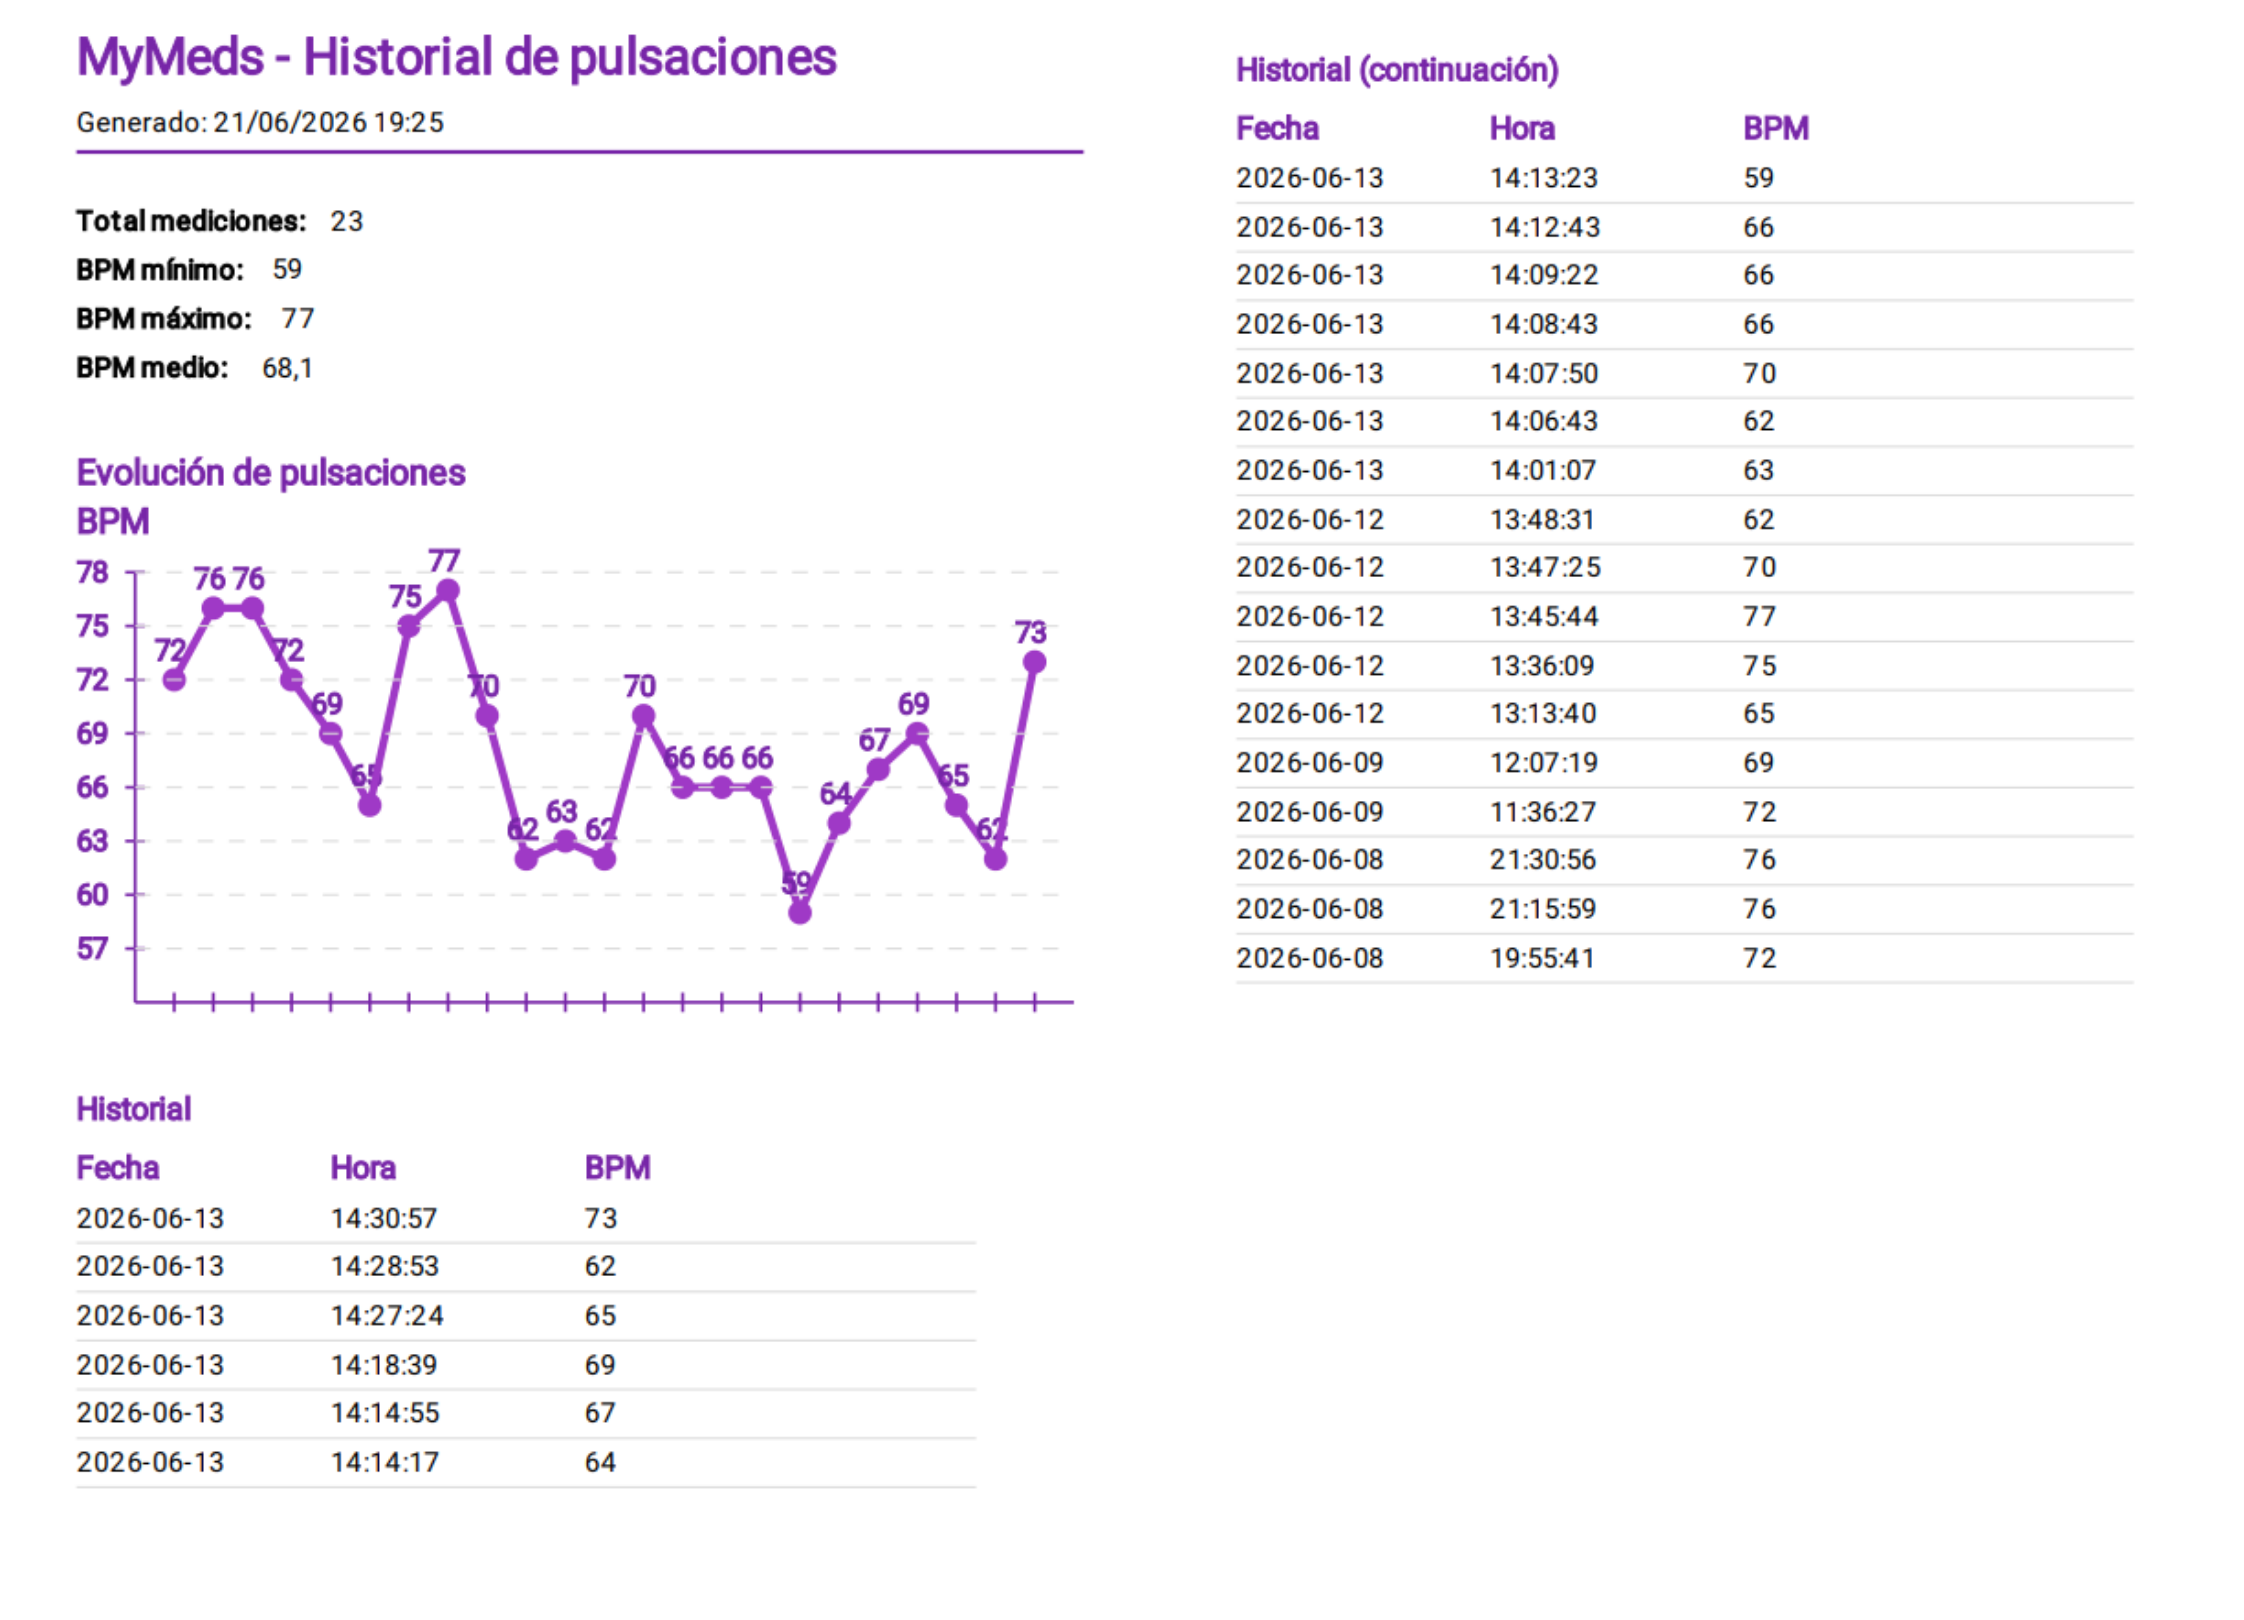
\includegraphics[width=0.6\textwidth]{figs/pdf_historial.png}
\caption{Informe PDF generado a partir del historial de mediciones almacenado.}
\label{fig:pdf}
\end{figure}

\

El desarrollo completo del experimento fue registrado en vídeo y puede consultarse en el enlace\footnote{\url{https://tinyurl.com/bdht27wc}}. Los resultados se resumen en la Tabla~\ref{tab}.

\begin{table}[H]
\centering
\caption{Resultados de la validación del historial de mediciones.}
\label{tab:historial_validacion}
\begin{tabular}{|l|c|}
\hline
\textbf{Prueba realizada} & \textbf{Resultado} \\ \hline
Almacenamiento de mediciones en fichero CSV & Correcto \\ \hline
Visualización del historial en el ESP32 & Correcto \\ \hline
Recuperación del historial desde Android & Correcto \\ \hline
Representación gráfica de las mediciones & Correcto \\ \hline
Generación de informe PDF & Correcto \\ \hline
Conservación del historial tras reinicio & Correcto \\ \hline
\end{tabular}
\end{table}

Los resultados obtenidos muestran que todas las mediciones realizadas fueron almacenadas correctamente en la tarjeta SD y permanecieron disponibles tras reiniciar el dispositivo. Asimismo, los datos pudieron recuperarse tanto desde la interfaz local implementada en el ESP32 como desde la aplicación Android desarrollada.\\

La correcta generación del informe PDF confirma, además, que la información almacenada puede ser procesada y exportada sin pérdidas de datos. En consecuencia, puede concluirse que los mecanismos de almacenamiento persistente y recuperación del historial implementados en el sistema funcionan de forma fiable y permiten conservar las mediciones realizadas para su posterior consulta y análisis.

\section{Seguridad del sistema}

Con el objetivo de restringir el acceso no autorizado y garantizar la correcta vinculación entre el dispositivo y la aplicación móvil, el sistema incorpora distintos mecanismos de seguridad. Entre ellos se incluyen un sistema de autenticación mediante PIN sincronizado entre ambos dispositivos, y un mecanismo de vinculación basado en tokens únicos. Para validar su funcionamiento se realizaron diferentes pruebas relacionadas con la autenticación de usuarios y la sincronización segura de la información.\\

\

\

\subsection{Validación del acceso mediante PIN}

Se implementó un mecanismo de autenticación basado en un PIN configurable por el usuario. Para validarlo se realizaron diferentes pruebas introduciendo tanto códigos correctos como incorrectos desde la aplicación móvil y desde el dispositivo.\\

Durante los ensayos se comprobó que el acceso únicamente era concedido cuando el PIN introducido coincidía con el almacenado en el sistema. En caso contrario, el acceso era denegado y el usuario permanecía en la pantalla de autenticación.\\

La Figura~\ref{fig:validacion_pin} muestra una captura correspondiente a una de las pruebas realizadas. El desarrollo completo de los ensayos de seguridad realizados en este apartado puede consultarse en el vídeo asociado\footnote{\url{https://tinyurl.com/4sy8tfjf}}. La grabación incluye simultáneamente la interfaz del dispositivo, la aplicación móvil y los registros de depuración generados por ambos sistemas, permitiendo observar en tiempo real los procesos de autenticación, sincronización del PIN y validación de las comunicaciones.

\begin{figure}[H]
\centering
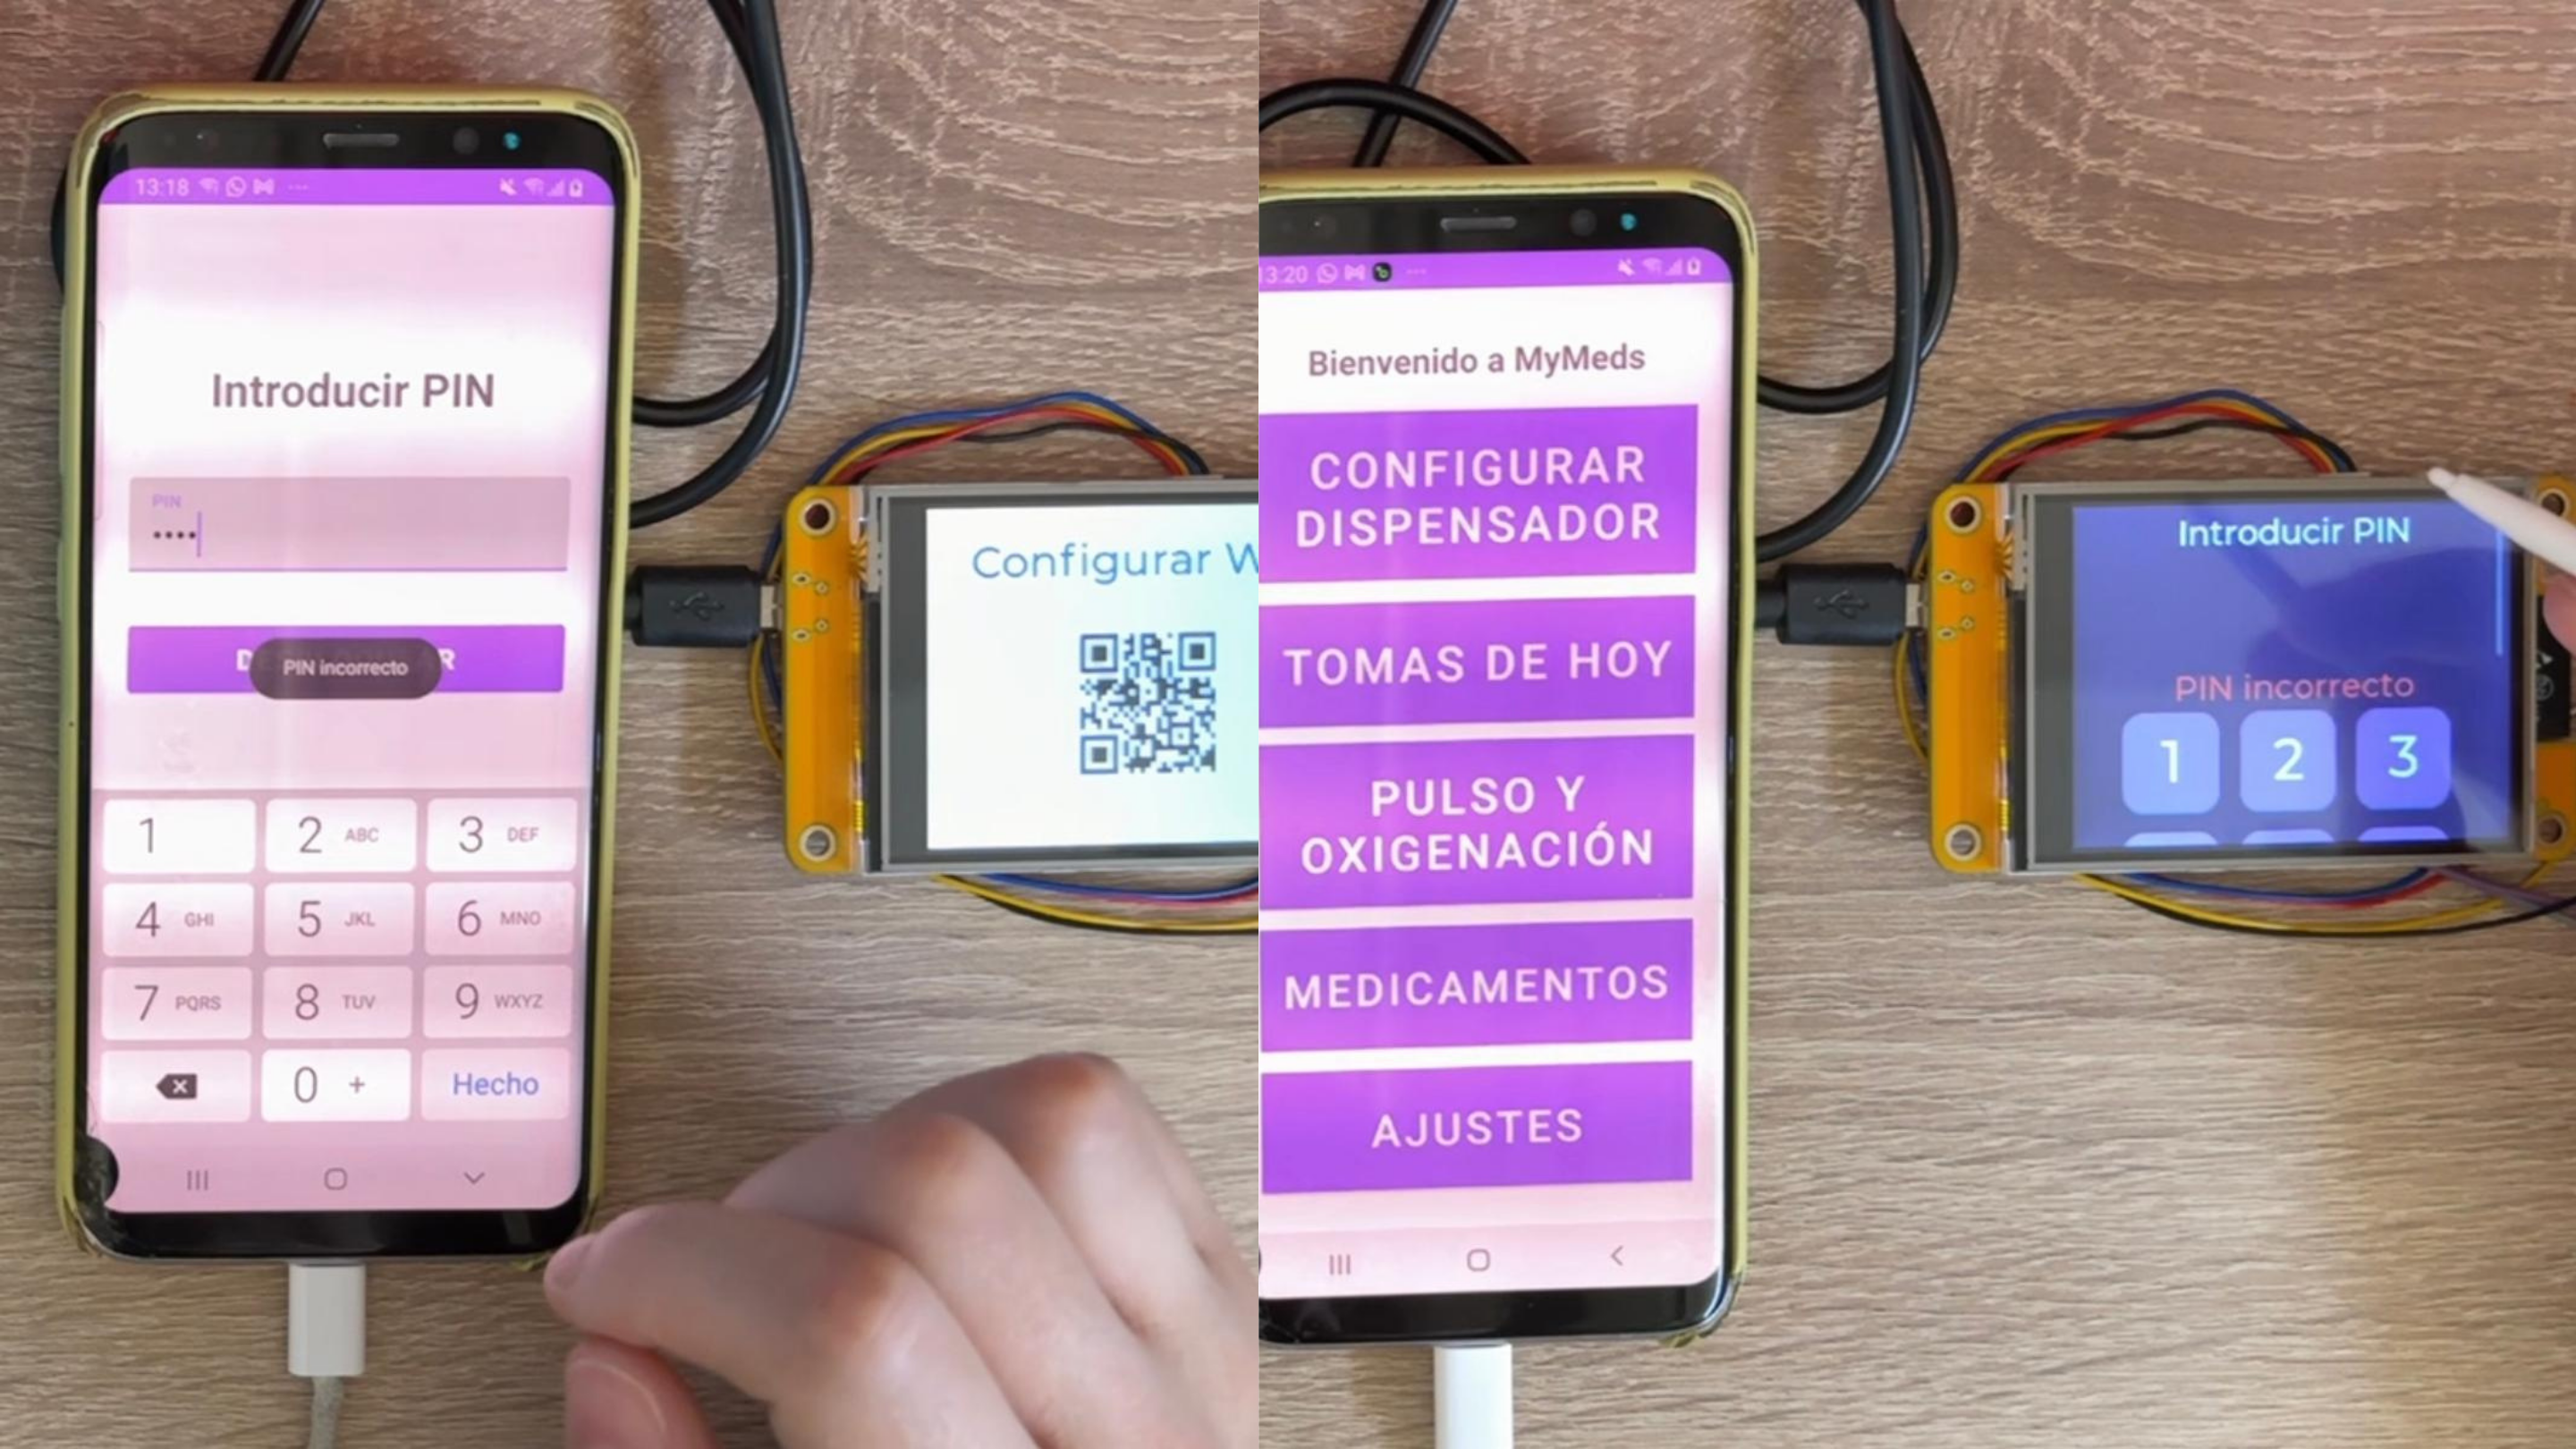
\includegraphics[width=0.8\textwidth]{figs/validacion_pin.png}
\caption{Validación del acceso mediante PIN.}
\label{fig:validacion_pin}
\end{figure}

\subsection{Sincronización del PIN}

El PIN de acceso, además de emplearse como mecanismo de autenticación, debe conservarse sincronizado entre el dispositivo y la aplicación móvil para asegurar que el sistema funcione de manera coherente. Con el fin de validar esta funcionalidad, se realizaron diferentes pruebas destinadas a comprobar que los cambios realizados sobre el código de autenticación se transmitían correctamente.

La metodología seguida consistió en modificar el PIN desde la aplicación móvil y verificar posteriormente que el nuevo valor era recibido y almacenado correctamente por el dispositivo. A continuación, se comprobó que el acceso mediante el PIN anterior era rechazado y que únicamente el nuevo código permitía desbloquear el sistema. Asimismo, se realizó un reinicio completo del dispositivo para verificar que el nuevo PIN se sincronizaría inmediatamente después del arranque.\\

Tal y como puede observarse en el vídeo\footnote{\url{https://tinyurl.com/4sy8tfjf}}, el proceso de actualización del PIN puede seguirse en tiempo real mediante los registros de depuración generados por la aplicación móvil y el ESP32. Estos registros permiten verificar la recepción del nuevo valor, su almacenamiento en el dispositivo y la posterior utilización del mismo durante el proceso de autenticación tras el reinicio del sistema.\\

La Figura~\ref{fig:sincronizacion_pin} muestra una captura correspondiente a una de las pruebas realizadas.

\begin{figure}[H]
\centering
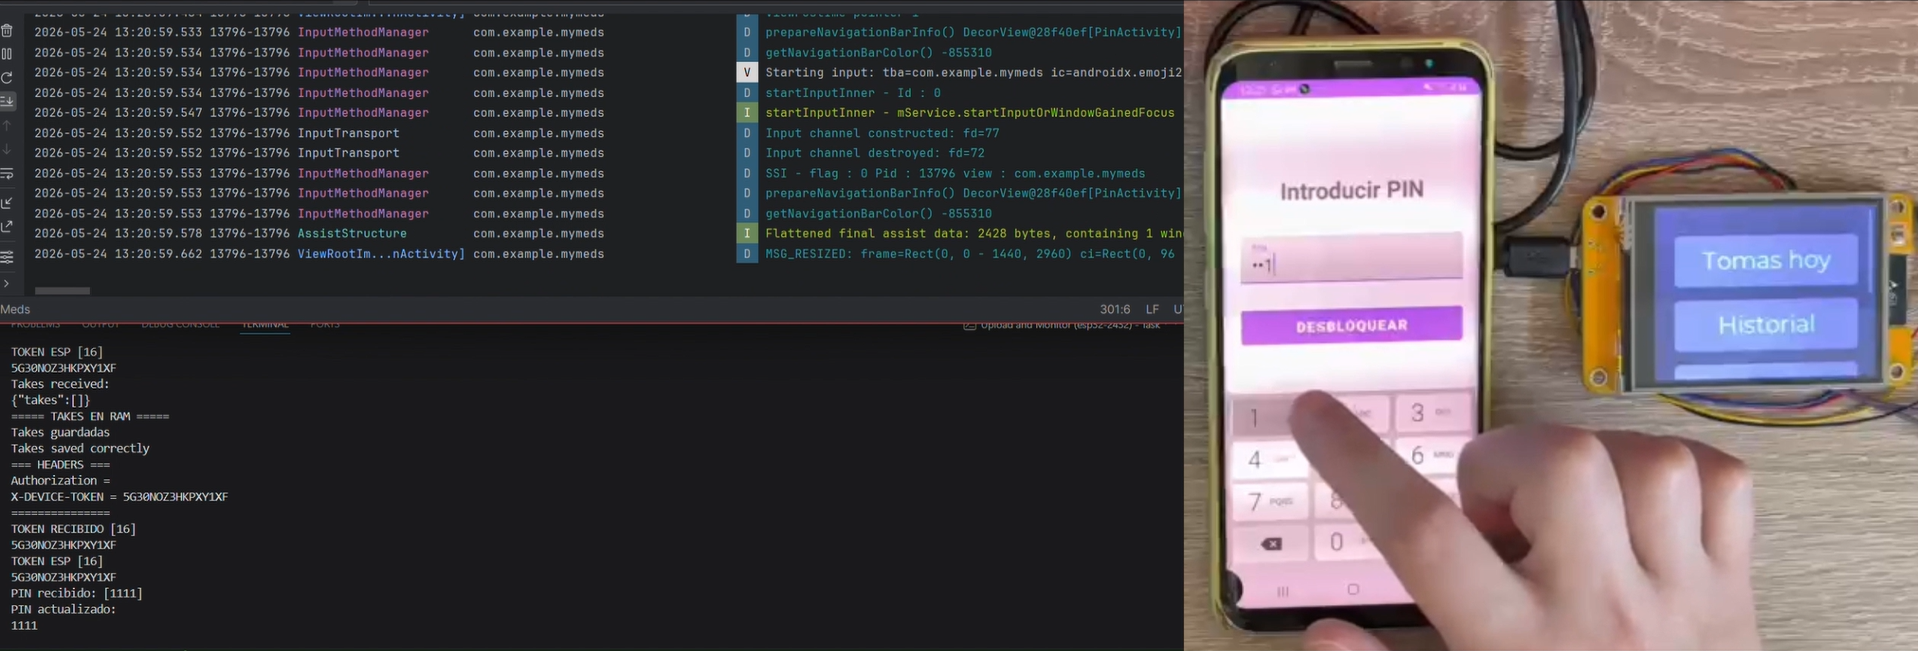
\includegraphics[width=\textwidth]{figs/sincronizacion_pin.png}
\caption{Validación de la sincronización del PIN entre app y dispositivo.}
\label{fig:sincronizacion_pin}
\end{figure}

Los resultados obtenidos se resumen en la Tabla~\ref{tab:sincronizacion_pin}.

\begin{table}[H]
\centering
\caption{Resultados de la validación de la sincronización del PIN.}
\label{tab:sincronizacion_pin}
\begin{tabular}{|l|c|}
\hline
\textbf{Prueba realizada} & \textbf{Resultado} \\ \hline
Actualización del PIN desde Android & Correcto \\ \hline
Recepción del nuevo PIN por el ESP32 & Correcto \\ \hline
Invalidación del PIN anterior & Correcto \\ \hline
Acceso mediante el nuevo PIN & Correcto \\ \hline
Persistencia tras reinicio & Correcto \\ \hline
\end{tabular}
\end{table}

\

\

Los experimentos realizados demuestran que el PIN sincronizado entre el dispositivo y la aplicación móvil funciona de manera adecuada. El valor nuevo fue reemplazado y guardado de manera exitosa después de cada cambio, y además permaneció accesible tras reiniciar el sistema. Esto asegura la consistencia de la configuración de seguridad y previene contradicciones entre ambos componentes.

\subsection{Sistema de vinculación mediante token}

Con el objetivo de evitar vinculaciones no autorizadas entre dispositivos, se implementó un mecanismo de emparejamiento basado en la generación y validación de tokens únicos. Este sistema permite garantizar que únicamente las aplicaciones autorizadas puedan establecer comunicaciones con el dispensador.\\

Para validar su funcionamiento se analizaron los intercambios de información producidos durante el proceso de vinculación entre la aplicación móvil y el dispositivo. Durante las pruebas se verificó que el sistema generaba correctamente un token de identificación aleatorio, que dicho token era transmitido a través de la comunicación establecida y que únicamente las solicitudes que incorporaban un token válido eran aceptadas por el dispositivo.\\

Tal y como puede observarse en el experimento descrito en los apartados anteriores, los registros de depuración mostrados simultáneamente por la aplicación móvil y el ESP32 permiten seguir en tiempo real el proceso de autorización. Gracias a ello fue posible verificar la correcta generación, transmisión y validación de los tokens utilizados durante la vinculación.\\

\begin{figure}[H]
\centering
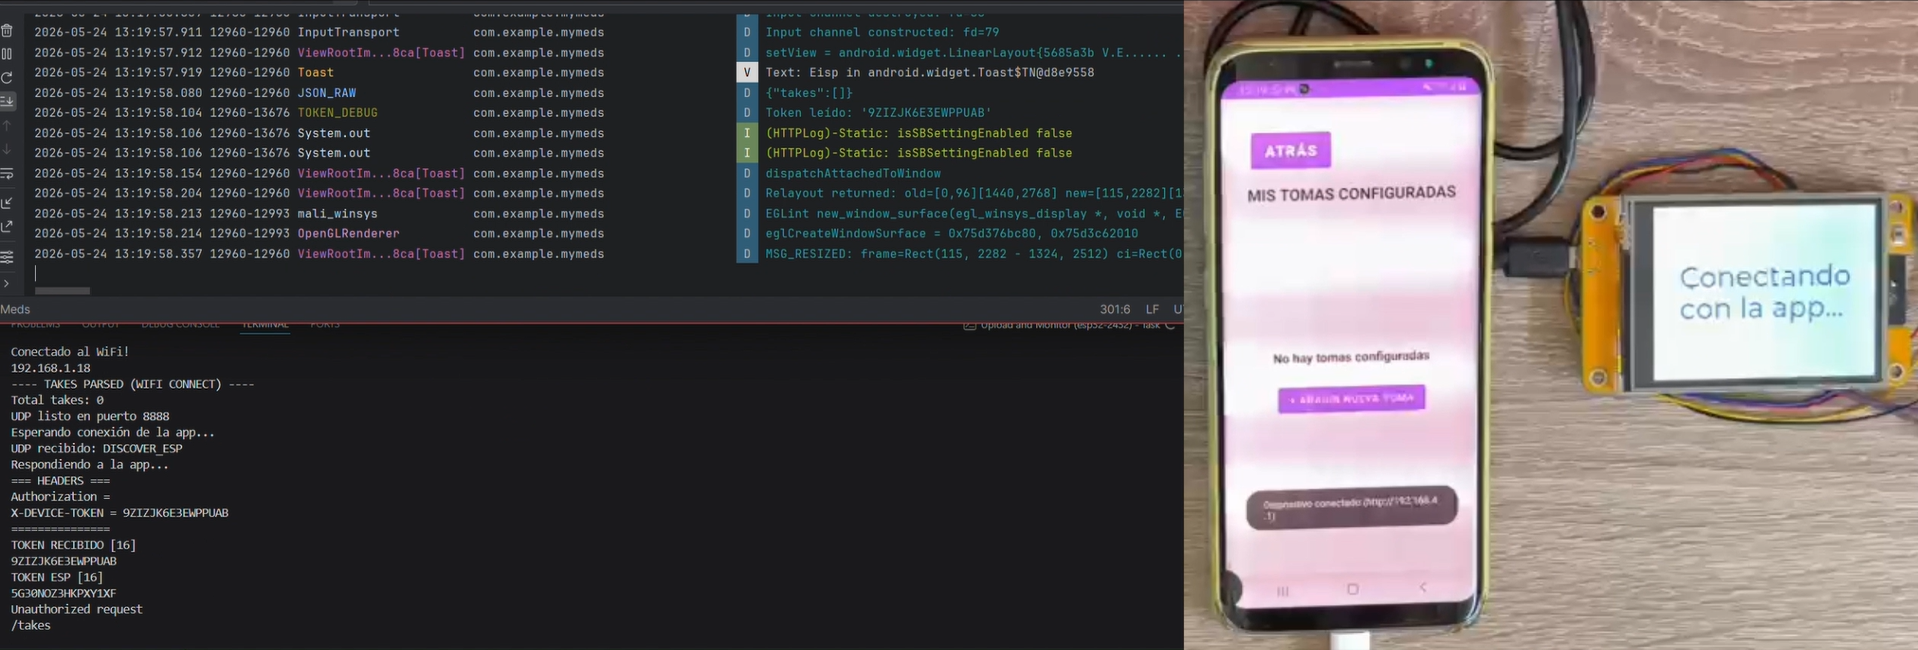
\includegraphics[width=\textwidth]{figs/token_vinculacion.png}
\caption{Mensajes de generación y validación del token en el proceso de vinculación.}
\label{fig:token_vinculacion}
\end{figure}

\

La Figura~\ref{fig:token_vinculacion} muestra una captura correspondiente a los mensajes de depuración registrados durante una de las pruebas realizadas. Asimismo, los resultados obtenidos se resumen en la Tabla~\ref{tab:token_vinculacion}.

\begin{table}[H]
\centering
\caption{Resultados de la validación del sistema de vinculación mediante token.}
\label{tab:token_vinculacion}
\begin{tabular}{|l|c|}
\hline
\textbf{Prueba realizada} & \textbf{Resultado} \\ \hline
Generación de token único & Correcto \\ \hline
Transmisión del token & Correcto \\ \hline
Validación del token & Correcto \\ \hline
Autorización de la vinculación & Correcto \\ \hline
\end{tabular}
\end{table}

Los ensayos realizados muestran que el mecanismo de vinculación implementado funciona correctamente, permitiendo identificar con certeza los dispositivos autorizados y evitando asociaciones no deseadas entre la aplicación móvil y el dispensador. Asimismo, la validación de los tokens garantiza que únicamente las comunicaciones autorizadas puedan acceder a las funcionalidades protegidas del sistema.

\section{Evaluación global del sistema}

Finalmente, se realizó una evaluación integral del sistema reproduciendo un escenario de uso representativo(Figura~\ref{fig:evaluacion_global}). Esta prueba permitió verificar el funcionamiento conjunto de los distintos módulos desarrollados y comprobar la correcta integración entre los componentes hardware y software que forman la solución propuesta.\\

La prueba consistió en recorrer el flujo completo de utilización del sistema, comenzando por el proceso de autenticación mediante PIN, la gestión de medicamentos y tomas desde la aplicación móvil, la sincronización bidireccional de la información, la medición de la frecuencia cardíaca, la consulta del historial de medidas, la generación del informe en formato PDF, y la dispensación automática de una toma programada. Asimismo, se comprobó la persistencia de la configuración tras reiniciar el dispositivo y la correcta recuperación de su estado.\\

El desarrollo completo de esta evaluación puede observarse en el vídeo asociado\footnote{\url{https://tinyurl.com/y2fv5dud}}.

\begin{figure}[H]
    \centering
    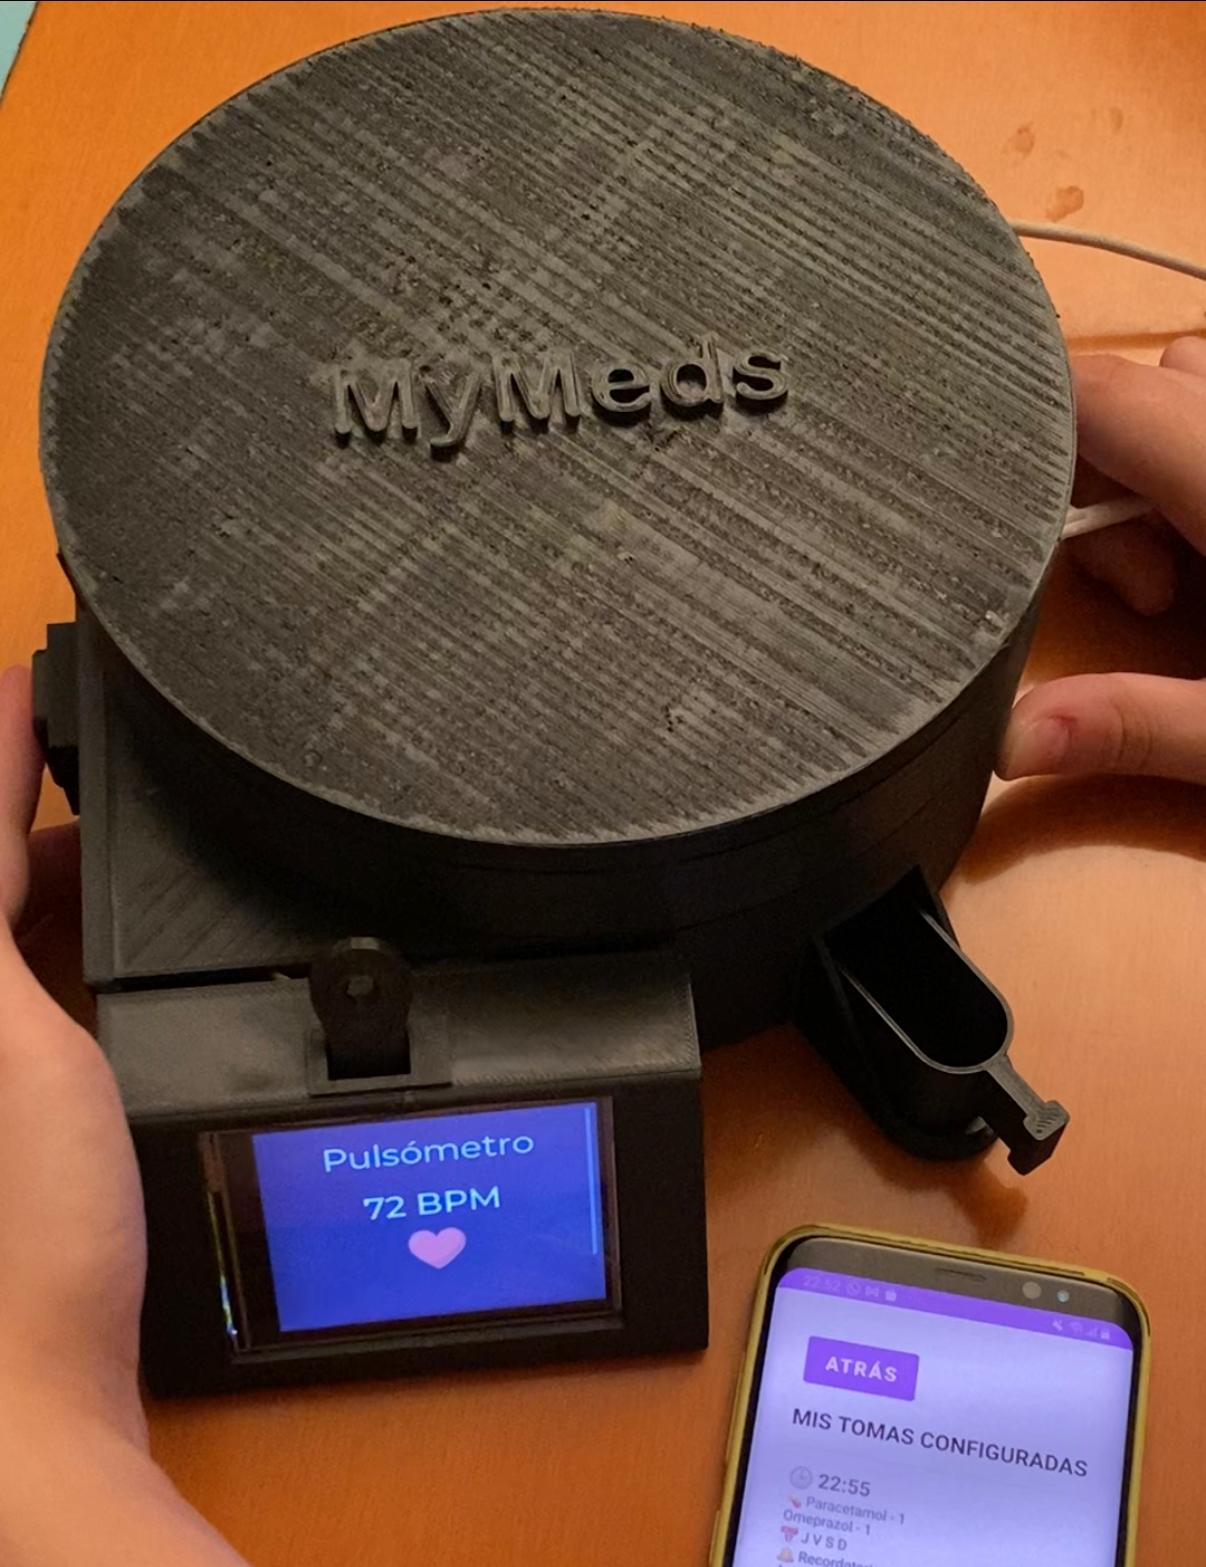
\includegraphics[width=0.5\linewidth]{figs/evaluacion_global.jpeg}
    \caption{Evaluación global del sistema MyMeds.}
    \label{fig:evaluacion_global}
\end{figure}

\begin{table}[H]
\centering
\caption{Resultados de la evaluación global del sistema.}
\label{tab:evaluacion_global}
\begin{tabular}{|p{9cm}|c|}
\hline
\textbf{Funcionalidad evaluada} & \textbf{Resultado} \\
\hline
Autenticación mediante PIN & Correcto \\
\hline
Gestión de medicamentos y tomas & Correcto \\
\hline
Sincronización bidireccional entre aplicación y dispositivo & Correcto \\
\hline
Medición y almacenamiento de pulsaciones & Correcto \\
\hline
Generación del informe PDF & Correcto \\
\hline
Dispensación automática de tomas programadas & Correcto \\
\hline
Persistencia de la configuración tras reinicio & Correcto \\
\hline
Funcionamiento autónomo del dispositivo & Correcto \\
\hline
\end{tabular}
\end{table}

Los resultados obtenidos, y mostrados en la Tabla~\ref{tab:evaluacion_global}, confirman que el sistema desarrollado integra correctamente todos los módulos hardware y software implementados, proporcionando un funcionamiento estable y coherente en un escenario de utilización real. Asimismo, las pruebas realizadas demuestran que \textit{MyMeds} satisface los requisitos funcionales definidos para el proyecto en la \autoref{sec:requisitos} y constituye una solución capaz de gestionar de forma autónoma la programación y dispensación de medicamentos, así como el registro y consulta de información biomédica.


